%%%%%%%%%%%%%%%%%%%%%%%%%%%%%%%%%%%%%%%%%%%%%%%%%%%%%%%%%%%%%%%%%%%%%%%%%%%%%%%%%%%%%%%%%%%
% Yet Another Thesis Template
% LuaLaTeX Template
%
% Source:
% https://github.com/alexpovel/thesis_template
%
% Original author:
% Alex Povel -- tex(at)alexpovel.de
%
% License and Copyright:
% MIT License
%
% Copyright (c) 2019 Alex Povel
%
% Permission is hereby granted, free of charge, to any person obtaining a copy
% of this software and associated documentation files (the "Software"), to deal
% in the Software without restriction, including without limitation the rights
% to use, copy, modify, merge, publish, distribute, sublicense, and/or sell
% copies of the Software, and to permit persons to whom the Software is
% furnished to do so, subject to the following conditions:
%
% The above copyright notice and this permission notice shall be included in all
% copies or substantial portions of the Software.
%
% THE SOFTWARE IS PROVIDED "AS IS", WITHOUT WARRANTY OF ANY KIND, EXPRESS OR
% IMPLIED, INCLUDING BUT NOT LIMITED TO THE WARRANTIES OF MERCHANTABILITY,
% FITNESS FOR A PARTICULAR PURPOSE AND NONINFRINGEMENT. IN NO EVENT SHALL THE
% AUTHORS OR COPYRIGHT HOLDERS BE LIABLE FOR ANY CLAIM, DAMAGES OR OTHER
% LIABILITY, WHETHER IN AN ACTION OF CONTRACT, TORT OR OTHERWISE, ARISING FROM,
% OUT OF OR IN CONNECTION WITH THE SOFTWARE OR THE USE OR OTHER DEALINGS IN THE
% SOFTWARE.
%
% Magic Comment:
% This template requires LuaLaTeX.
% The following 'magic comment' is recognized by editors and will ensure lualatex engine use:
%!TEX TS-program = lualatex
%%%%%%%%%%%%%%%%%%%%%%%%%%%%%%%%%%%%%%%%%%%%%%%%%%%%%%%%%%%%%%%%%%%%%%%%%%%%%%%%%%%%%%%%%%%
\documentclass[compress, english]{beamer}% Compress chapter overview in header
%%%%%%%%%%%%%%%%%%%%%%%%%%%%%%%%%%%%%%%%%%%%%%%%%%%%%%%%%%%%%%%%%%%%%%%%%%%%%%%%%%%%%%%%%%%
%%%%%%%%%%%%%%%%%%%%%%%%%%%%%%%%%%%%%%%%%%%%%%%%%%%%%%%%%%%%%%%%%%%%%%%%%%%%%%%%%%%%%%%%%%%
% Yet Another Thesis Template
% LuaLaTeX Template
%
% Source:
% https://github.com/alexpovel/thesis_template
%
% Original author:
% Alex Povel -- tex(at)alexpovel.de
%
% License and Copyright:
% MIT License
%
% Copyright (c) 2019 Alex Povel
%
% Permission is hereby granted, free of charge, to any person obtaining a copy
% of this software and associated documentation files (the "Software"), to deal
% in the Software without restriction, including without limitation the rights
% to use, copy, modify, merge, publish, distribute, sublicense, and/or sell
% copies of the Software, and to permit persons to whom the Software is
% furnished to do so, subject to the following conditions:
%
% The above copyright notice and this permission notice shall be included in all
% copies or substantial portions of the Software.
%
% THE SOFTWARE IS PROVIDED "AS IS", WITHOUT WARRANTY OF ANY KIND, EXPRESS OR
% IMPLIED, INCLUDING BUT NOT LIMITED TO THE WARRANTIES OF MERCHANTABILITY,
% FITNESS FOR A PARTICULAR PURPOSE AND NONINFRINGEMENT. IN NO EVENT SHALL THE
% AUTHORS OR COPYRIGHT HOLDERS BE LIABLE FOR ANY CLAIM, DAMAGES OR OTHER
% LIABILITY, WHETHER IN AN ACTION OF CONTRACT, TORT OR OTHERWISE, ARISING FROM,
% OUT OF OR IN CONNECTION WITH THE SOFTWARE OR THE USE OR OTHER DEALINGS IN THE
% SOFTWARE.
%
% Magic Comment:
% This template requires LuaLaTeX.
% The following 'magic comment' is recognized by editors and will ensure lualatex engine use:
%!TEX TS-program = lualatex
%%%%%%%%%%%%%%%%%%%%%%%%%%%%%%%%%%%%%%%%%%%%%%%%%%%%%%%%%%%%%%%%%%%%%%%%%%%%%%%%%%%%%%%%%%%
%%%%%%%%%%%%%% The presentation preamble shares a lot of content with the regular thesis
%%%%%%%%%%%%%% preamble. However, joining both and creating a 'shared preamble' was found
%%%%%%%%%%%%%% to be pretty error-prone.
%%%%%%%%%%%%%% Using overlapping but distinct preamble files allows for two stand-alone
%%%%%%%%%%%%%% documents.
%%%%%%%%%%%%%%%%%%%%%%%%%%%%%%%%%%%%%%%%%%%%%%%%%%%%%%%%%%%%%%%%%%%%%%%%%%%%%%%%%%%%%%%%%%%
%%%%%%%%%%%%%%%%%%%%%%%%%%%%%%%%%%%%%%%%%%%%%%%%%%%%%%%%%%%%%%%%%%%%%%%%%%%%%%%%%%%%%%%%%%%
%%%%%%%%%%%%%%%%%%%%%%%%%%%%%%%%%%%%%%%%%%%%%%%%%%%%%%%%%%%%%%%%%%%%%%%%%%%%%%%%%%%%%%%%%%%
%%%%%%%%%%%%%%%%%%%%%%%%%%%%%%%%%%%%%%%%%%%%%%%%%%%%%%%%%%%%%%%%%%%%%%%%%%%%%%%%%%%%%%%%%%%
%%%%%%%%%%%%%% Typography and Misc.
%%%%%%%%%%%%%%%%%%%%%%%%%%%%%%%%%%%%%%%%%%%%%%%%%%%%%%%%%%%%%%%%%%%%%%%%%%%%%%%%%%%%%%%%%%%
%%%%%%%%%%%%%%%%%%%%%%%%%%%%%%%%%%%%%%%%%%%%%%%%%%%%%%%%%%%%%%%%%%%%%%%%%%%%%%%%%%%%%%%%%%%
%%%%%%%%%%%%%%%%%%%%%%%%%%%%%%%%%%%%%%%%%%%%%%%%%%%%%%%%%%%%%%%%%%%%%%%%%%%%%%%%%%%%%%%%%%%
%\usepackage{showframe}% Debugging
\usepackage{kantlipsum}% Debugging
%%%%%%%%%%%%%%%%%%%%%%%%%%%%%%%%%%%%%%%%%%%%%%%%%%%%%%%%%%%%%%%%%%%%%%%%%%%%%%%%%%%%%%%%%%%
\usepackage{amsmath}% Required before fontspec/unicode-math
\usepackage{mathtools}% AMSmath extension; coloneqq etc.
%%%%%%%%%%%%%%%%%%%%%%%%%%%%%%%%%%%%%%%%%%%%%%%%%%%%%%%%%%%%%%%%%%%%%%%%%%%%%%%%%%%%%%%%%%%
%%%%%%%%%%%%%%%%%%%%%%%%%%%%%%%%%%%%%%%%%%%%%%%%%%%%%%%%%%%%%%%%%%%%%%%%%%%%%%%%%%%%%%%%%%%
%%%%%%%%%%%%%% Theme: https://github.com/matze/mtheme
%%%%%%%%%%%%%%%%%%%%%%%%%%%%%%%%%%%%%%%%%%%%%%%%%%%%%%%%%%%%%%%%%%%%%%%%%%%%%%%%%%%%%%%%%%%
%%%%%%%%%%%%%%%%%%%%%%%%%%%%%%%%%%%%%%%%%%%%%%%%%%%%%%%%%%%%%%%%%%%%%%%%%%%%%%%%%%%%%%%%%%%
\usetheme[%
sectionpage=none,%
titleformat frame=smallcaps,%
]{metropolis}%
%%%%%%%%%%%%%%%%%%%%%%%%%%%%%%%%%%%%%%%%%%%%%%%%%%%%%%%%%%%%%%%%%%%%%%%%%%%%%%%%%%%%%%%%%%%
%%%%%%%%%%%%%%%%%%%%%%%%%%%%%%%%%%%%%%%%%%%%%%%%%%%%%%%%%%%%%%%%%%%%%%%%%%%%%%%%%%%%%%%%%%%
%%%%%%%%%%%%%% Presentation aka beamer-specific settings
%%%%%%%%%%%%%%%%%%%%%%%%%%%%%%%%%%%%%%%%%%%%%%%%%%%%%%%%%%%%%%%%%%%%%%%%%%%%%%%%%%%%%%%%%%%
%%%%%%%%%%%%%%%%%%%%%%%%%%%%%%%%%%%%%%%%%%%%%%%%%%%%%%%%%%%%%%%%%%%%%%%%%%%%%%%%%%%%%%%%%%%
% Global default overlay specification for enumerate/itemize/actionenv etc.:
\beamerdefaultoverlayspecification{<+->}%
\setbeamercovered{highly dynamic}% Make uncovering very dynamic
%%%%%%%%%%%%%%%%%%%%%%%%%%%%%%%%%%%%%%%%%%%%%%%%%%%%%%%%%%%%%%%%%%%%%%%%%%%%%%%%%%%%%%%%%%%
\usepackage{appendixnumberbeamer}% Fix totalframenumber so that appendix doesn't count
%%%%%%%%%%%%%%%%%%%%%%%%%%%%%%%%%%%%%%%%%%%%%%%%%%%%%%%%%%%%%%%%%%%%%%%%%%%%%%%%%%%%%%%%%%%
%%%%%%%%%%%%%% Outer theme sets navigational elements/header/footer/sidebar
%%%%%%%%%%%%%%%%%%%%%%%%%%%%%%%%%%%%%%%%%%%%%%%%%%%%%%%%%%%%%%%%%%%%%%%%%%%%%%%%%%%%%%%%%%%
\useoutertheme[subsection=false]{miniframes}
\setbeamercolor{section in head/foot}{fg=normal text.bg, bg=structure.fg}% Outer theme colors
%%%%%%%%%%%%%%%%%%%%%%%%%%%%%%%%%%%%%%%%%%%%%%%%%%%%%%%%%%%%%%%%%%%%%%%%%%%%%%%%%%%%%%%%%%%
%%%%%%%%%%%%%% Numbers and indentation in ToC
%%%%%%%%%%%%%%%%%%%%%%%%%%%%%%%%%%%%%%%%%%%%%%%%%%%%%%%%%%%%%%%%%%%%%%%%%%%%%%%%%%%%%%%%%%%
\setbeamertemplate{section in toc}[sections numbered]%
\setbeamertemplate{subsection in toc}%
{\leavevmode\leftskip=3.2em\rlap{\hskip-2em\inserttocsectionnumber.\inserttocsubsectionnumber}\inserttocsubsection\par}% https://tex.stackexchange.com/a/371613/120853
%%%%%%%%%%%%%%%%%%%%%%%%%%%%%%%%%%%%%%%%%%%%%%%%%%%%%%%%%%%%%%%%%%%%%%%%%%%%%%%%%%%%%%%%%%%
%%%%%%%%%%%%%% Commands to exclude certain frames from *.nav-file/navigation bar
%%%%%%%%%%%%%%%%%%%%%%%%%%%%%%%%%%%%%%%%%%%%%%%%%%%%%%%%%%%%%%%%%%%%%%%%%%%%%%%%%%%%%%%%%%%
% https://tex.stackexchange.com/a/45038/120853
\makeatletter
\let\beamer@writeslidentry@miniframeson=\beamer@writeslidentry
\def\beamer@writeslidentry@miniframesoff{%
	\expandafter\beamer@ifempty\expandafter{\beamer@framestartpage}{}% does not happen normally
	{%else
		% removed \addtocontents commands
		\clearpage\beamer@notesactions%
	}
}
\newcommand*{\miniframeson}{\let\beamer@writeslidentry=\beamer@writeslidentry@miniframeson}
\newcommand*{\miniframesoff}{\let\beamer@writeslidentry=\beamer@writeslidentry@miniframesoff}
\makeatother
%%%%%%%%%%%%%%%%%%%%%%%%%%%%%%%%%%%%%%%%%%%%%%%%%%%%%%%%%%%%%%%%%%%%%%%%%%%%%%%%%%%%%%%%%%%
%%%%%%%%%%%%%% Print an overview with current subsection highlighted at each subsection start
%%%%%%%%%%%%%%%%%%%%%%%%%%%%%%%%%%%%%%%%%%%%%%%%%%%%%%%%%%%%%%%%%%%%%%%%%%%%%%%%%%%%%%%%%%%
\AtBeginSubsection[]{% Empty brackets: do nothing for \subsection*
	{%
		\setbeamertemplate{footline}{}% Hide footer/pagenumber; can't use plain style because we want to keep headline
		\miniframesoff
		\begin{frame}<handout:0>[noframenumbering]{Agenda}
			\tableofcontents[%
			currentsection,% Highlight this
			currentsubsection,% Highlight this
			subsectionstyle=show/shaded/hide,%https://tex.stackexchange.com/a/193981/120853
			]%
		\end{frame}%
		\miniframeson
	}%
}
%%%%%%%%%%%%%%%%%%%%%%%%%%%%%%%%%%%%%%%%%%%%%%%%%%%%%%%%%%%%%%%%%%%%%%%%%%%%%%%%%%%%%%%%%%%
\AtBeginSection[]{% Empty brackets: do nothing for \section*
	{%
		\setbeamertemplate{footline}{}% Hide footer/pagenumber; can't use plain style because we want to keep headline
		\miniframesoff
		\begin{frame}<handout:0>[noframenumbering]{Agenda}
			\tableofcontents[%
			currentsection,% Highlight this
			%currentsubsection,% Highlight this
			subsectionstyle=show/shaded/hide,%https://tex.stackexchange.com/a/193981/120853
			]%
		\end{frame}%
		\miniframeson
	}%
}
%%%%%%%%%%%%%%%%%%%%%%%%%%%%%%%%%%%%%%%%%%%%%%%%%%%%%%%%%%%%%%%%%%%%%%%%%%%%%%%%%%%%%%%%%%%
%%%%%%%%%%%%%% Other settings
%%%%%%%%%%%%%%%%%%%%%%%%%%%%%%%%%%%%%%%%%%%%%%%%%%%%%%%%%%%%%%%%%%%%%%%%%%%%%%%%%%%%%%%%%%%
% Put a square as the item, immitating what we did in the thesis.
% We can't use unicode-math symbols, so just put a small rectangle (a \rule)
% Beamer+enumitem together are problematic: https://tex.stackexchange.com/a/24491/120853
\setbeamertemplate{itemize items}{\raisebox{0.35ex}{\rule{0.55ex}{0.55ex}}}%[square]% All three levels; beamer-default [square] is too large
%%%%%%%%%%%%%%%%%%%%%%%%%%%%%%%%%%%%%%%%%%%%%%%%%%%%%%%%%%%%%%%%%%%%%%%%%%%%%%%%%%%%%%%%%%%
%%%%%%%%%%%%%%%%%%%%%%%%%%%%%%%%%%%%%%%%%%%%%%%%%%%%%%%%%%%%%%%%%%%%%%%%%%%%%%%%%%%%%%%%%%%
%%%%%%%%%%%%%% Typography and Misc.
%%%%%%%%%%%%%%%%%%%%%%%%%%%%%%%%%%%%%%%%%%%%%%%%%%%%%%%%%%%%%%%%%%%%%%%%%%%%%%%%%%%%%%%%%%%
%%%%%%%%%%%%%%%%%%%%%%%%%%%%%%%%%%%%%%%%%%%%%%%%%%%%%%%%%%%%%%%%%%%%%%%%%%%%%%%%%%%%%%%%%%%
%%%%%%%%%%%%%% Thoughts on fonts:
%%%%%%%%%%%%%% metropolis theme has issues with math font (https://github.com/matze/mtheme/issues/263)
%%%%%%%%%%%%%% The current default/best solution is to use Computer Modern; doesn't look good
%%%%%%%%%%%%%% Solution: use high-quality math font. Available as FiraMath, which is in beta.
%%%%%%%%%%%%%% It works rather well, but has bugs (e.g. with \dot not centered hor., subscripts too low)
%%%%%%%%%%%%%% Alternative: use packages of matching non-Fira fonts for math (https://tex.stackexchange.com/q/403734/120853)
%%%%%%%%%%%%%% 1. 'arevmath' looks too bold. Setting the text-fonts bolder seems unacceptable, they look very nice in the original metropolis theme and should remain unchanged
%%%%%%%%%%%%%% 2. 'eulervm' is also bugged with \dot (https://tex.stackexchange.com/q/50273/120853)
%%%%%%%%%%%%%% 3. newtxsf seems okay for now (https://tex.stackexchange.com/questions/422415/fira-sans-math-companion#comment1056174_422415)
%%%%%%%%%%%%%% Author of newtxsf package recommends it to go along with FiraSans, see their doc.
%%%%%%%%%%%%%%%%%%%%%%%%%%%%%%%%%%%%%%%%%%%%%%%%%%%%%%%%%%%%%%%%%%%%%%%%%%%%%%%%%%%%%%%%%%%
%%%%%%%%%%%%%%%%%%%%%%%%%%%%%%%%%%%%%%%%%%%%%%%%%%%%%%%%%%%%%%%%%%%%%%%%%%%%%%%%%%%%%%%%%%%
%%%%%%%%%%%%%% Uncomment this block for unicode-math font specs.
%%%%%%%%%%%%%% Currently not used because of beta-status of Fira Math.
%%%%%%%%%%%%%% We don't set a roman/main font because that should never be used in presentations.
%\usefonttheme{professionalfonts}% Prevent Beamer from overriding if high-quality fonts are used
%\usepackage{unicode-math}% Requires Unicode font input
%%%%%%%%%%%%%% Be specific with font specifications so that it's clear what happens.
%%%%%%%%%%%%%% No funny business, full control, high guarantee of compatibility across machines and time.
%\defaultfontfeatures{Path=fonts/, Extension=.otf}% All fonts
%\setsansfont[% https://tex.stackexchange.com/a/62605/120853
%	Ligatures=TeX,%
%	Path=fonts/Fira/Sans/Normal/,
%	UprightFont={*-Light},% Put Light weight as actual font
%	ItalicFont={*-LightItalic},%
%	BoldFont={*-Regular},%
%	BoldItalicFont={*-Italic}]%
%	{FiraSans}%[Color=B3EB83]% Toggle color for debugging
%\setmonofont[%
%	Path=fonts/Fira/Mono/,%
%	UprightFont={*-Regular},%
%	BoldFont={*-Medium},% Mono has weight: Regular/Medium/Bold
%	]%
%	{FiraMono}%[Color=FFCE5B]% Toggle color for debugging
%\setmathfont[%
%	Path=fonts/Fira/Math/,%
%	mathrm=sym,%set math-font-commands to new versions
%	mathit=sym,%
%	mathsf=sym,%
%	mathbf=sym,%
%	mathtt=sym]%
%	{FiraMath-Light}%[Color=E85748]% Toggle color for debugging
%%%%%%%%%%%%%%%%%%%%%%%%%%%%%%%%%%%%%%%%%%%%%%%%%%%%%%%%%%%%%%%%%%%%%%%%%%%%%%%%%%%%%%%%%%%
%%%%%%%%%%%%%%%%%%%%%%%%%%%%%%%%%%%%%%%%%%%%%%%%%%%%%%%%%%%%%%%%%%%%%%%%%%%%%%%%%%%%%%%%%%%
\usepackage{newtxsf}% For math, matches Fira Sans text font
%%%%%%%%%%%%%%%%%%%%%%%%%%%%%%%%%%%%%%%%%%%%%%%%%%%%%%%%%%%%%%%%%%%%%%%%%%%%%%%%%%%%%%%%%%%
%%%%%%%%%%%%%%%%%%%%%%%%%%%%%%%%%%%%%%%%%%%%%%%%%%%%%%%%%%%%%%%%%%%%%%%%%%%%%%%%%%%%%%%%%%%
%%%%%%%%%%%%%% System Information Banner
%%%%%%%%%%%%%%%%%%%%%%%%%%%%%%%%%%%%%%%%%%%%%%%%%%%%%%%%%%%%%%%%%%%%%%%%%%%%%%%%%%%%%%%%%%%
\usepackage{hologo}
% Using fontspec, this document is incompatible with anything but XeLaTeX/LuaLaTeX.
% LuaLaTeX can grab additional memory as needed, therefore no issues with tikz and
% no need to tikzexternalize.
% Further, contour-package and XeLaTeX are strictly incompatible (LuaLaTeX works).
% Therefore, only ever use LuaLaTeX anyway.
\usepackage{xstring}
% Print only what occurs after 'This is ' and store in macro.
% luatexbanner is provided by luatex engine.
% https://tex.stackexchange.com/a/394043/120853
\StrBehind*{\luatexbanner}{This is }[\shortbanner]
% Take input and substitute strings, in this case make plain LuaTeX string into pretty logo.
% StrSubstitue has no starred variant, therefore dekotenize.
% https://tex.stackexchange.com/a/350583/120853
\StrSubstitute{\shortbanner}{\detokenize{LuaTeX}}{\hologo{LuaTeX}}[\prettybanner]

% Get contents of files
\usepackage{catchfile}
% Store textfile data in macro.
% If required, e.g. if the build process does not involve replacing the defaults
% with current values, set defaults in that file.
\CatchFileDef{\gitmetafile}{gitmeta.txt}{}
% Store result in new expandable macro, since xstring cmds are unexpandable.
% https://tex.stackexchange.com/a/476839/120853
\StrBetween[1,1]{\gitmetafile}{version=}{;}[\GitVersion]
\StrBetween[1,2]{\gitmetafile}{shorthash=}{;}[\GitShorthash]
%%%%%%%%%%%%%%%%%%%%%%%%%%%%%%%%%%%%%%%%%%%%%%%%%%%%%%%%%%%%%%%%%%%%%%%%%%%%%%%%%%%%%%%%%%%
%%%%%%%%%%%%%%%%%%%%%%%%%%%%%%%%%%%%%%%%%%%%%%%%%%%%%%%%%%%%%%%%%%%%%%%%%%%%%%%%%%%%%%%%%%%
%%%%%%%%%%%%%% Language
%%%%%%%%%%%%%%%%%%%%%%%%%%%%%%%%%%%%%%%%%%%%%%%%%%%%%%%%%%%%%%%%%%%%%%%%%%%%%%%%%%%%%%%%%%%
%%%%%%%%%%%%%%%%%%%%%%%%%%%%%%%%%%%%%%%%%%%%%%%%%%%%%%%%%%%%%%%%%%%%%%%%%%%%%%%%%%%%%%%%%%%
\usepackage{polyglossia}% Language rules. Replacement for babel in lualatex
	\setmainlanguage[variant=uk]{english}

\usepackage[style=british]{csquotes}

\usepackage[useregional]{datetime2}% Replaces 'datetime'

\usepackage{microtype}% Advanced typesetting

\usepackage{ragged2e}% For \justifying in the Abstract

\usepackage{booktabs}% For beautiful tables; absolute must
%%%%%%%%%%%%%%%%%%%%%%%%%%%%%%%%%%%%%%%%%%%%%%%%%%%%%%%%%%%%%%%%%%%%%%%%%%%%%%%%%%%%%%%%%%%
%%%%%%%%%%%%%%%%%%%%%%%%%%%%%%%%%%%%%%%%%%%%%%%%%%%%%%%%%%%%%%%%%%%%%%%%%%%%%%%%%%%%%%%%%%%
%%%%%%%%%%%%%% Auxiliary
%%%%%%%%%%%%%%%%%%%%%%%%%%%%%%%%%%%%%%%%%%%%%%%%%%%%%%%%%%%%%%%%%%%%%%%%%%%%%%%%%%%%%%%%%%%
%%%%%%%%%%%%%%%%%%%%%%%%%%%%%%%%%%%%%%%%%%%%%%%%%%%%%%%%%%%%%%%%%%%%%%%%%%%%%%%%%%%%%%%%%%%
\usepackage{scalerel}% Scale stuff relative

\newcommand*{\scaletox}[1]{\scalerel*{\includegraphics{./logos/#1.pdf}}{X}}%logos to Xheight

\newcommand*{\simplecross}{\scaletox{cross}}
%%%%%%%%%%%%%%%%%%%%%%%%%%%%%%%%%%%%%%%%%%%%%%%%%%%%%%%%%%%%%%%%%%%%%%%%%%%%%%%%%%%%%%%%%%%
\usepackage{array}
	\newcolumntype{M}[1]{>{\centering\arraybackslash}m{#1}}% Vert.+Hor. centering
%%%%%%%%%%%%%%%%%%%%%%%%%%%%%%%%%%%%%%%%%%%%%%%%%%%%%%%%%%%%%%%%%%%%%%%%%%%%%%%%%%%%%%%%%%%%
\usepackage[outline]{contour}% Incomptatible with xelatex
	\contourlength{0.15em}% default width is not 'strong' enough
	\newcommand*{\ctrw}[1]{\hypersetup{hidelinks}\contour{bg}{#1}}% bg colour
%%%%%%%%%%%%%%%%%%%%%%%%%%%%%%%%%%%%%%%%%%%%%%%%%%%%%%%%%%%%%%%%%%%%%%%%%%%%%%%%%%%%%%%%%%%
\usepackage{hyperref}% Loads URL-package internally
\hypersetup{%
pdfpagelayout=SinglePage,% Presentations aren't TwoPage etc.
unicode,%https://tex.stackexchange.com/a/66771/120853
pdfsubject = {Your Subject},%
pdfkeywords = {Your Keywords},%
}%
\usepackage[% biber is default backend
	style=numeric-comp,% Compress numeric into ranges
	autocite=superscript,% Behaviour of all \autocite commands
	sorting=none,% None: process in order of citation, so that we have counting up from 1
	sortcites=true,% Sortcites sorts multiple \cite-entries the way the sorting-key dictates
%	backref=slide,%https://tex.stackexchange.com/a/211631/120853. Do not use hyperref for this!
	url=false,% Still prints URL for @online
	doi=false,%
	isbn=false,%
	]{biblatex}%
\addbibresource{yatt.bib}% *.bib file w/ file-suffix goes here
%%%%%%%%%%%%%%%%%%%%%%%%%%%%%%%%%%%%%%%%%%%%%%%%%%%%%%%%%%%%%%%%%%%%%%%%%%%%%%%%%%%%%%%%%%%
%%%%%%%%%%%%%% Color citations; previously: https://tex.stackexchange.com/a/165016/120853
%%%%%%%%%%%%%%%%%%%%%%%%%%%%%%%%%%%%%%%%%%%%%%%%%%%%%%%%%%%%%%%%%%%%%%%%%%%%%%%%%%%%%%%%%%%
\AtEveryCite{\color{black!40}}% https://tex.stackexchange.com/a/258415/120853
%%%%%%%%%%%%%%%%%%%%%%%%%%%%%%%%%%%%%%%%%%%%%%%%%%%%%%%%%%%%%%%%%%%%%%%%%%%%%%%%%%%%%%%%%%%
%%%%%%%%%%%%%%%%%%%%%%%%%%%%%%%%%%%%%%%%%%%%%%%%%%%%%%%%%%%%%%%%%%%%%%%%%%%%%%%%%%%%%%%%%%%
%%%%%%%%%%%%%% Math, Science etc.
%%%%%%%%%%%%%%%%%%%%%%%%%%%%%%%%%%%%%%%%%%%%%%%%%%%%%%%%%%%%%%%%%%%%%%%%%%%%%%%%%%%%%%%%%%%
%%%%%%%%%%%%%%%%%%%%%%%%%%%%%%%%%%%%%%%%%%%%%%%%%%%%%%%%%%%%%%%%%%%%%%%%%%%%%%%%%%%%%%%%%%%
\usepackage{chemformula}
\usepackage{siunitx}
	\sisetup{%
		detect-weight,% Detect surrounding font's weight
		per-mode=symbol,% symbol: kg/(s), as opposed to kgs^-1 (so we take up less space)
		unit-mode=text,% Always print in text-font (so no italics)
	}%

%\usepackage{physics}% If you can, don't use it: https://tex.stackexchange.com/q/471532/120853

\DeclareMathOperator{\Mach}{M}
%%%%%%%%%%%%%%%%%%%%%%%%%%%%%%%%%%%%%%%%%%%%%%%%%%%%%%%%%%%%%%%%%%%%%%%%%%%%%%%%%%%%%%%%%%%
%%%%%%%%%%%%%% Visuals and Graphics
%%%%%%%%%%%%%%%%%%%%%%%%%%%%%%%%%%%%%%%%%%%%%%%%%%%%%%%%%%%%%%%%%%%%%%%%%%%%%%%%%%%%%%%%%%%
\usepackage{graphicx}
	\graphicspath{{images/}}%
\usepackage{xcolor}
	% colorbrewer modified RdYlBu:
	\definecolor{rdylbu1}{RGB}{215, 48, 39}% Red
	\definecolor{rdylbu2}{RGB}{252, 141, 89}%
	\definecolor{rdylbu3}{RGB}{254, 224, 144}%
	\definecolor{rdylbu4}{RGB}{224, 243, 248}%
	\definecolor{rdylbu5}{RGB}{145, 191, 219}%
	\definecolor{rdylbu6}{RGB}{69, 117, 180}% Blue

	\definecolor{mBlue}{RGB}{124, 196, 240}% Stronger blue than in thesis to match stronger orange of metropolis theme; bit hacky
%%%%%%%%%%%%%%%%%%%%%%%%%%%%%%%%%%%%%%%%%%%%%%%%%%%%%%%%%%%%%%%%%%%%%%%%%%%%%%%%%%%%%%%%%%%
%%%%%%%%%%%%%% Tikz + Plots
%%%%%%%%%%%%%%%%%%%%%%%%%%%%%%%%%%%%%%%%%%%%%%%%%%%%%%%%%%%%%%%%%%%%%%%%%%%%%%%%%%%%%%%%%%%
\usepackage{pgfplots}

\usetikzlibrary{%
positioning,%
calc,%
tikzmark,%
arrows,
backgrounds,%
shapes,% 'regular polygon'
fit}

\usepgfplotslibrary{%
groupplots,%
units,%
}%
%%%%%%%%%%%%%%%%%%%%%%%%%%%%%%%%%%%%%%%%%%%%%%%%%%%%%%%%%%%%%%%%%%%%%%%%%%%%%%%%%%%%%%%%%%%
%%%%%%%%%%%%%% Colour Cycle for plots
%%%%%%%%%%%%%%%%%%%%%%%%%%%%%%%%%%%%%%%%%%%%%%%%%%%%%%%%%%%%%%%%%%%%%%%%%%%%%%%%%%%%%%%%%%%
\pgfplotscreateplotcyclelist{mod RdYlBu3}{%modify existing colorbrewer
	{mLightBrown},% mLightBrown as defined in metropolis theme
	{mBlue},% mDarkTeal as defined in metropolis theme
	{mDarkTeal}%no comma here
}%
\pgfplotscreateplotcyclelist{mod mark list}{%modify predefined to start without mark
every mark/.append style={solid,fill=\pgfplotsmarklistfill}\\
every mark/.append style={solid,fill=\pgfplotsmarklistfill},mark=*\\
every mark/.append style={solid,fill=\pgfplotsmarklistfill},mark=square*\\
every mark/.append style={solid,fill=\pgfplotsmarklistfill},mark=triangle*\\
every mark/.append style={solid},mark=star\\
every mark/.append style={solid,fill=\pgfplotsmarklistfill},mark=diamond*\\
every mark/.append style={solid,fill=\pgfplotsmarklistfill!40},mark=otimes*\\
every mark/.append style={solid},mark=|\\
every mark/.append style={solid,fill=\pgfplotsmarklistfill},mark=pentagon*\\
}%
%%%%%%%%%%%%%%%%%%%%%%%%%%%%%%%%%%%%%%%%%%%%%%%%%%%%%%%%%%%%%%%%%%%%%%%%%%%%%%%%%%%%%%%%%%%
%%%%%%%%%%%%%% Global plot settings
%%%%%%%%%%%%%%%%%%%%%%%%%%%%%%%%%%%%%%%%%%%%%%%%%%%%%%%%%%%%%%%%%%%%%%%%%%%%%%%%%%%%%%%%%%%
\pgfplotstableset{col sep=comma}%if ALL files are comma-sep
\pgfplotsset{%
compat = newest,%
axis lines=left,%
cycle multi list = {%
	mod mark list\nextlist%just in case; likely never reached
	linestyles*\nextlist
	mod RdYlBu3%iterate through this first; if at end, start anew using next in parent
	},%
%
unit code/.code 2 args={\si{#1#2}},% Use siunitx for units library
unit markings = {slash space},
x SI prefix/micro/.style={/pgfplots/axis base prefix={axis x base 6 prefix \micro}},% https://tex.stackexchange.com/a/224574/120853
y SI prefix/micro/.style={/pgfplots/axis base prefix={axis y base 6 prefix \micro}},
z SI prefix/micro/.style={/pgfplots/axis base prefix={axis z base 6 prefix \micro}},
%
group style = {%
	xticklabels at = edge bottom,
	xlabels at = edge bottom,
	vertical sep = 3ex,
	group size = 1 by 2,
},%
%
tuftelike/.style={%https://tex.stackexchange.com/a/155210/120853
	axis line shift=10pt,% Also shifts label
	axis line style={-},
	try min ticks=3,% https://tex.stackexchange.com/a/95753/120853
	max space between ticks=50,%
},%
minimalistic/.style={%
	tuftelike,
	thick,
	axis line style = semithick,
	tick style = {semithick, fg},% fg is current beamer foreground color
	width=0.35\textwidth,
	height=0.4\textheight,
	ytick align=inside,%puts ticks inside the plot itself
	xtick align=inside,%
	title style = {font=\footnotesize},
	xtick={% Always set min, max and middle ticks; if more desired, use 'extra x ticks={}'
		\pgfkeysvalueof{/pgfplots/xmin},
		\pgfkeysvalueof{/pgfplots/xmax},
		(\pgfkeysvalueof{/pgfplots/xmax}+\pgfkeysvalueof{/pgfplots/xmin})/2
	},
	ytick={% Same as x
		\pgfkeysvalueof{/pgfplots/ymin},
		\pgfkeysvalueof{/pgfplots/ymax},
		(\pgfkeysvalueof{/pgfplots/ymax}+\pgfkeysvalueof{/pgfplots/ymin})/2
	},
	clip = false,% https://tex.stackexchange.com/a/311194/120853
	label style={font=\tiny},%https://tex.stackexchange.com/a/300673/120853
	tick label style={font=\tiny, /pgf/number format/1000 sep={\,}},%
},%
invisible/.style={opacity=0},% https://tex.stackexchange.com/a/269558/120853
visible on/.style={alt={#1{}{invisible}}},
alt/.code args={<#1>#2#3}{%
	\alt<#1>{\pgfkeysalso{#2}}{\pgfkeysalso{#3}} % \pgfkeysalso doesn't change the path
},
}%
\tikzstyle{simblock} = [%
	draw,%
	line width=1.5pt,%
	minimum size = 1.5em,%
	rounded corners,%
	fill = white,%
	]%
\tikzstyle{triangle} = [%https://tex.stackexchange.com/a/183092/120853
	regular polygon,%
	regular polygon sides=3,%
	inner sep = 0.2ex,%fit tightly
	outer sep = 0pt,
	]%
%%%%%%%%%%%%%%%%%%%%%%%%%%%%%%%%%%%%%%%%%%%%%%%%%%%%%%%%%%%%%%%%%%%%%%%%%%%%%%%%%%%%%%%%%%%
%%%%%%%%%%%%%% Functions for plotting
%%%%%%%%%%%%%%%%%%%%%%%%%%%%%%%%%%%%%%%%%%%%%%%%%%%%%%%%%%%%%%%%%%%%%%%%%%%%%%%%%%%%%%%%%%%
\tikzset{declare function={%https://tex.stackexchange.com/a/279234/120853
cpm(\x)= (\x<=500) * (0.781*(28.98641+1.853978*((\x+273.15)/1000)-9.647459*((\x+273.15)/1000)^2+16.63537*((\x+273.15)/1000)^3+0.000117/(((\x+273.15)/1000)^2))+0.2093*(31.32234-20.23531*((\x+273.15)/1000)+57.86644*((\x+273.15)/1000)^2-36.50624*((\x+273.15)/1000)^3-0.007374/((\x+273.15)/1000)^2)  +0.0093*(20.78600+2.825911e-7*((\x+273.15)/1000)-1.464191e-7*((\x+273.15)/1000)^2+1.092131e-8*((\x+273.15)/1000)^3-3.661371e-8/((\x+273.15)/1000)^2)+0.0004*(24.99735+55.18696*((\x+273.15)/1000)-33.69137*((\x+273.15)/1000)^2+7.948387*((\x+273.15)/1000)^3-0.136638/((\x+273.15)/1000)^2)) +
(\x>500) * (0.781*(19.50583+19.88705*((\x+273.15)/1000)-8.598535*((\x+273.15)/1000)^2+1.369784*((\x+273.15)/1000)^3+0.527691/(((\x+273.15)/1000)^2))+0.2093*(31.32234-20.23531*((\x+273.15)/1000)+57.86644*((\x+273.15)/1000)^2-36.50624*((\x+273.15)/1000)^3-0.007374/((\x+273.15)/1000)^2)+0.0093*(20.78600+2.825911e-7*((\x+273.15)/1000)-1.464191e-7*((\x+273.15)/1000)^2+1.092131e-8*((\x+273.15)/1000)^3-3.661371e-8/((\x+273.15)/1000)^2)+0.0004*(24.99735+55.18696*((\x+273.15)/1000)-33.69137*((\x+273.15)/1000)^2+7.948387*((\x+273.15)/1000)^3-0.136638/((\x+273.15)/1000)^2));%SHOMATE
muoxy(\x) = 20.8e-6 * (300 + 127)/(\x + 127) * (\x / 300)^(3/2);%viscosity oxygen (mu oxygen)
%
munit(\x) = 17.9e-6 * (300 + 111)/(\x + 111) * (\x / 300)^(3/2);%viscosity nitrogen (mu nitrogen)
%
muar(\x) = 22.9e-6 * (300 + 170)/(\x + 170) * (\x / 300)^(3/2);%viscosity argon (mu argon)
%
mucoo(\x) = 15e-6 * (300 + 240)/(\x + 240) * (\x / 300)^(3/2);%viscosity carbon dioxide (mu coo)
},%
}%
%%%%%%%%%%%%%%%%%%%%%%%%%%%%%%%%%%%%%%%%%%%%%%%%%%%%%%%%%%%%%%%%%%%%%%%%%%%%%%%%%%%%%%%%%%%
%%%%%%%%%%%%%%%%%%%%%%%%%%%%%%%%%%%%%%%%%%%%%%%%%%%%%%%%%%%%%%%%%%%%%%%%%%%%%%%%%%%%%%%%%%%
%%%%%%%%%%%%%% Glossaries; dont use for presentations, but nice for consistent symbols etc
%%%%%%%%%%%%%%%%%%%%%%%%%%%%%%%%%%%%%%%%%%%%%%%%%%%%%%%%%%%%%%%%%%%%%%%%%%%%%%%%%%%%%%%%%%%
%%%%%%%%%%%%%%%%%%%%%%%%%%%%%%%%%%%%%%%%%%%%%%%%%%%%%%%%%%%%%%%%%%%%%%%%%%%%%%%%%%%%%%%%%%%
\usepackage[abbreviations, symbols, record, nomain]{glossaries-extra}
% Record for bib2gls to work.
% Nomain, aka no default glossary
% Also see https://tex.stackexchange.com/q/477658/120853
%%%%%%%%%%%%%%%%%%%%%%%%%%%%%%%%%%%%%%%%%%%%%%%%%%%%%%%%%%%%%%%%%%%%%%%%%%%%%%%%%%%%%%%%%%%
%%%%%%%%%%%%%% New Glossary 'types'. Load data into them from *.bib-files, then run bib2gls
%%%%%%%%%%%%%%%%%%%%%%%%%%%%%%%%%%%%%%%%%%%%%%%%%%%%%%%%%%%%%%%%%%%%%%%%%%%%%%%%%%%%%%%%%%%
% Using Abbreviations/Symbols package options creates these glossaries already.
% Create the rest manually.
\newglossary*{subsuper}{Sub- and Superscripts}%
\GlsXtrLoadResources[%
	src={./glossaries/abbreviations},%
	selection = {all},% Enable for debugging
]%
\GlsXtrLoadResources[%
	src={./glossaries/symbols},%
	selection = {all},% Enable for debugging
]%
\GlsXtrLoadResources[%
	src={./glossaries/subsuper},%
	type=subsuper,%
	category = subsuper,
	selection = {all},% Enable for debugging
]%
% Disable hyperlinking in presentation:
\glsdisablehyper
%%%%%%%%%%%%%%%%%%%%%%%%%%%%%%%%%%%%%%%%%%%%%%%%%%%%%%%%%%%%%%%%%%%%%%%%%%%%%%%%%%%%%%%%%%%
%%%%%%%%%%%%%%%%%%%%%%%%%%%%%%%%%%%%%%%%%%%%%%%%%%%%%%%%%%%%%%%%%%%%%%%%%%%%%%%%%%%%%%%%%%%
%%%%%%%%%%%%%% Custom Commands
%%%%%%%%%%%%%%%%%%%%%%%%%%%%%%%%%%%%%%%%%%%%%%%%%%%%%%%%%%%%%%%%%%%%%%%%%%%%%%%%%%%%%%%%%%%
%%%%%%%%%%%%%%%%%%%%%%%%%%%%%%%%%%%%%%%%%%%%%%%%%%%%%%%%%%%%%%%%%%%%%%%%%%%%%%%%%%%%%%%%%%%
% In the original thesis document, \name is used alongside \sindex to produce index entries for all names; in order to use it here, too, define it but remove index capabilities:
\newcommand*{\name}[1]{\textsc{#1}}% Just a wrapper for people's names
%%%%%%%%%%%%%%%%%%%%%%%%%%%%%%%%%%%%%%%%%%%%%%%%%%%%%%%%%%%%%%%%%%%%%%%%%%%%%%%%%%%%%%%%%%%
\newcommand*{\whitebox}[1]{\setlength{\fboxsep}{3pt}\colorbox{bg}{#1}} %https://tex.stackexchange.com/a/23682/120853
%%%%%%%%%%%%%%%%%%%%%%%%%%%%%%%%%%%%%%%%%%%%%%%%%%%%%%%%%%%%%%%%%%%%%%%%%%%%%%%%%%%%%%%%%%%
\newcommand*{\angstanitz}[1]{\ensuremath{\gls{angabs}_{#1}^{\ast}}}%Stanitz shifted by 90deg
%%%%%%%%%%%%%%%%%%%%%%%%%%%%%%%%%%%%%%%%%%%%%%%%%%%%%%%%%%%%%%%%%%%%%%%%%%%%%%%%%%%%%%%%%%%
\newcommand*{\const}{const.}%
%%%%%%%%%%%%%%%%%%%%%%%%%%%%%%%%%%%%%%%%%%%%%%%%%%%%%%%%%%%%%%%%%%%%%%%%%%%%%%%%%%%%%%%%%%%
%%%%%%%%%%%%%% Tikz
%%%%%%%%%%%%%%%%%%%%%%%%%%%%%%%%%%%%%%%%%%%%%%%%%%%%%%%%%%%%%%%%%%%%%%%%%%%%%%%%%%%%%%%%%%%
\newcommand*{\circnum}[1]{% A circled (preferably) number
%	\tikzset{external/export=false}% Never externalize this
	\tikz[baseline=(X.base)]%
	\node (X) [draw, shape=circle, inner sep=1pt, fill=bg] {\textbf{#1}};%
}%
\newcommand*{\circlet}[1]{% A circled letter
%	\tikzset{external/export=false}% Never externalize
	\tikz[baseline=(char.base)]{%
	\node [draw, shape=circle, inner sep=1pt, fill=bg] (char) {\textbf{#1}};}%
}%
%%%%%%%%%%%%%%%%%%%%%%%%%%%%%%%%%%%%%%%%%%%%%%%%%%%%%%%%%%%%%%%%%%%%%%%%%%%%%%%%%%%%%%%%%%%
%%%%%%%%%%%%%% Vectors
%%%%%%%%%%%%%%%%%%%%%%%%%%%%%%%%%%%%%%%%%%%%%%%%%%%%%%%%%%%%%%%%%%%%%%%%%%%%%%%%%%%%%%%%%%%
% The bib2gls library (*.bib-files) uses \symbf etc. from unicode-math, since
% the thesis documents is based on that package. The presentation here is not,
% therefore we provide the command manually, so the bib-files are usable.
\providecommand*{\symbf}{\mathbf}
\newcommand*{\vect}[2]{\ensuremath{\vec{\symbf{#1}}_{\text{#2}}}}% Vector
\newcommand*{\vectcomp}[3]{\ensuremath{\symbf{#1}_{\text{#2#3}}}}% Vector component
%%%%%%%%%%%%%%%%%%%%%%%%%%%%%%%%%%%%%%%%%%%%%%%%%%%%%%%%%%%%%%%%%%%%%%%%%%%%%%%%%%%%%%%%%%%
%%%%%%%%%%%%%% Physics-package-like commands
%%%%%%%%%%%%%%%%%%%%%%%%%%%%%%%%%%%%%%%%%%%%%%%%%%%%%%%%%%%%%%%%%%%%%%%%%%%%%%%%%%%%%%%%%%%
% Physics package has problems. E.g., \dd prints roman -> poor for sans-serif presentation
%\providecommand{\var}[1]{\ensuremath{\delta #1}}%
\providecommand{\dd}[1]{\ensuremath{\textnormal{d}#1}}%
%%%%%%%%%%%%%%%%%%%%%%%%%%%%%%%%%%%%%%%%%%%%%%%%%%%%%%%%%%%%%%%%%%%%%%%%%%%%%%%%%%%%%%%%%%%
%%%%%%%%%%%%%% Programs/Languages
%%%%%%%%%%%%%%%%%%%%%%%%%%%%%%%%%%%%%%%%%%%%%%%%%%%%%%%%%%%%%%%%%%%%%%%%%%%%%%%%%%%%%%%%%%%
\newcommand*{\smlnk}{%https://tex.stackexchange.com/a/471263/120853
	Simulink%
	\nobreak
	\textsuperscript{\textregistered}%
}%
\newcommand*{\mtlb}{%
	MATLAB%
	\nobreak
	\textsuperscript{\textregistered}%
}%
\newcommand*{\mtlbsymb}{%
	Symbolic Math Toolbox%
	\nobreak
	\textsuperscript{\texttrademark}%
}%
\newcommand*{\mtlbsmlnk}{%
	\mtlb % MATLAB
	\kern-0.25em % move the slash back
	\slash % allow a break after the slash
	\nobreak % the next space is not allowed for a break
	\hspace{0pt}% allow the next word to be hyphenated
	\smlnk
}%
\newcommand*{\smscp}{%
	Simscape%
	\nobreak%
	\textsuperscript{\texttrademark}%
}%
\newcommand*{\fortran}{%
FORTRAN\term{FORTRAN}%
}%%
%%%%%%%%%%%%%%%%%%%%%%%%%%%%%%%%%%%%%%%%%%%%%%%%%%%%%%%%%%%%%%%%%%%%%%%%%%%%%%%%%%%%%%%%%%%
% Label a slide 'current' and toggle here for speed; comment line to process entire document
%\includeonlyframes{title, debugging, current}%
%%%%%%%%%%%%%%%%%%%%%%%%%%%%%%%%%%%%%%%%%%%%%%%%%%%%%%%%%%%%%%%%%%%%%%%%%%%%%%%%%%%%%%%%%%%
%%%%%%%%%%%%%%%%%%%%%%%%%%%%%%%%%%%%%%%%%%%%%%%%%%%%%%%%%%%%%%%%%%%%%%%%%%%%%%%%%%%%%%%%%%%
%%%%%%%%%%%%%% Titlepage and document metadata content:
%%%%%%%%%%%%%%%%%%%%%%%%%%%%%%%%%%%%%%%%%%%%%%%%%%%%%%%%%%%%%%%%%%%%%%%%%%%%%%%%%%%%%%%%%%%
%%%%%%%%%%%%%%%%%%%%%%%%%%%%%%%%%%%%%%%%%%%%%%%%%%%%%%%%%%%%%%%%%%%%%%%%%%%%%%%%%%%%%%%%%%%
\title{The title of your very nice and highly important, never before seen scientific work of stellar excellence}
% An example on how to use datetime2 'objects'.
% Read documentation, put in date in appropriate format,
% it then gets printed according to your chosen locale (in preamble).
% No more fiddling around or inconsistency.
\date{\DTMdate{2021-03-12}}
\author{Your Name}
\institute{Your amazing university!}
\subtitle{Possibly a subtitle}
%%%%%%%%%%%%%%%%%%%%%%%%%%%%%%%%%%%%%%%%%%%%%%%%%%%%%%%%%%%%%%%%%%%%%%%%%%%%%%%%%%%%%%%%%%%
%%%%%%%%%%%%%%%%%%%%%%%%%%%%%%%%%%%%%%%%%%%%%%%%%%%%%%%%%%%%%%%%%%%%%%%%%%%%%%%%%%%%%%%%%%%
\begin{document}
\begin{frame}<handout:0>[label=title,noframenumbering,plain]
\maketitle
\end{frame}
%%%%%%%%%%%%%%%%%%%%%%%%%%%%%%%%%%%%%%%%%%%%%%%%%%%%%%%%%%%%%%%%%%%%%%%%%%%%%%%%%%%%%%%%%%%
\begin{frame}<handout:0>[label=attention-getter,plain,noframenumbering,standout]{}
A brief teaser to get attention!
\end{frame}
%%%%%%%%%%%%%%%%%%%%%%%%%%%%%%%%%%%%%%%%%%%%%%%%%%%%%%%%%%%%%%%%%%%%%%%%%%%%%%%%%%%%%%%%%%%
\begin{frame}<handout:0>[label=upshot]{Upshot}
{\footnotesize Tell them what the end result of your work is! Generally, use as little ink and as many graphical elements as possible.}

\centering
\visible<+->{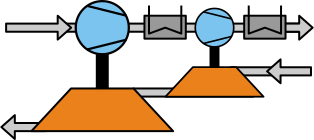
\includegraphics[width=0.35\textwidth]{turbo_series_pres}}%
\hspace{5em}
\visible<+->{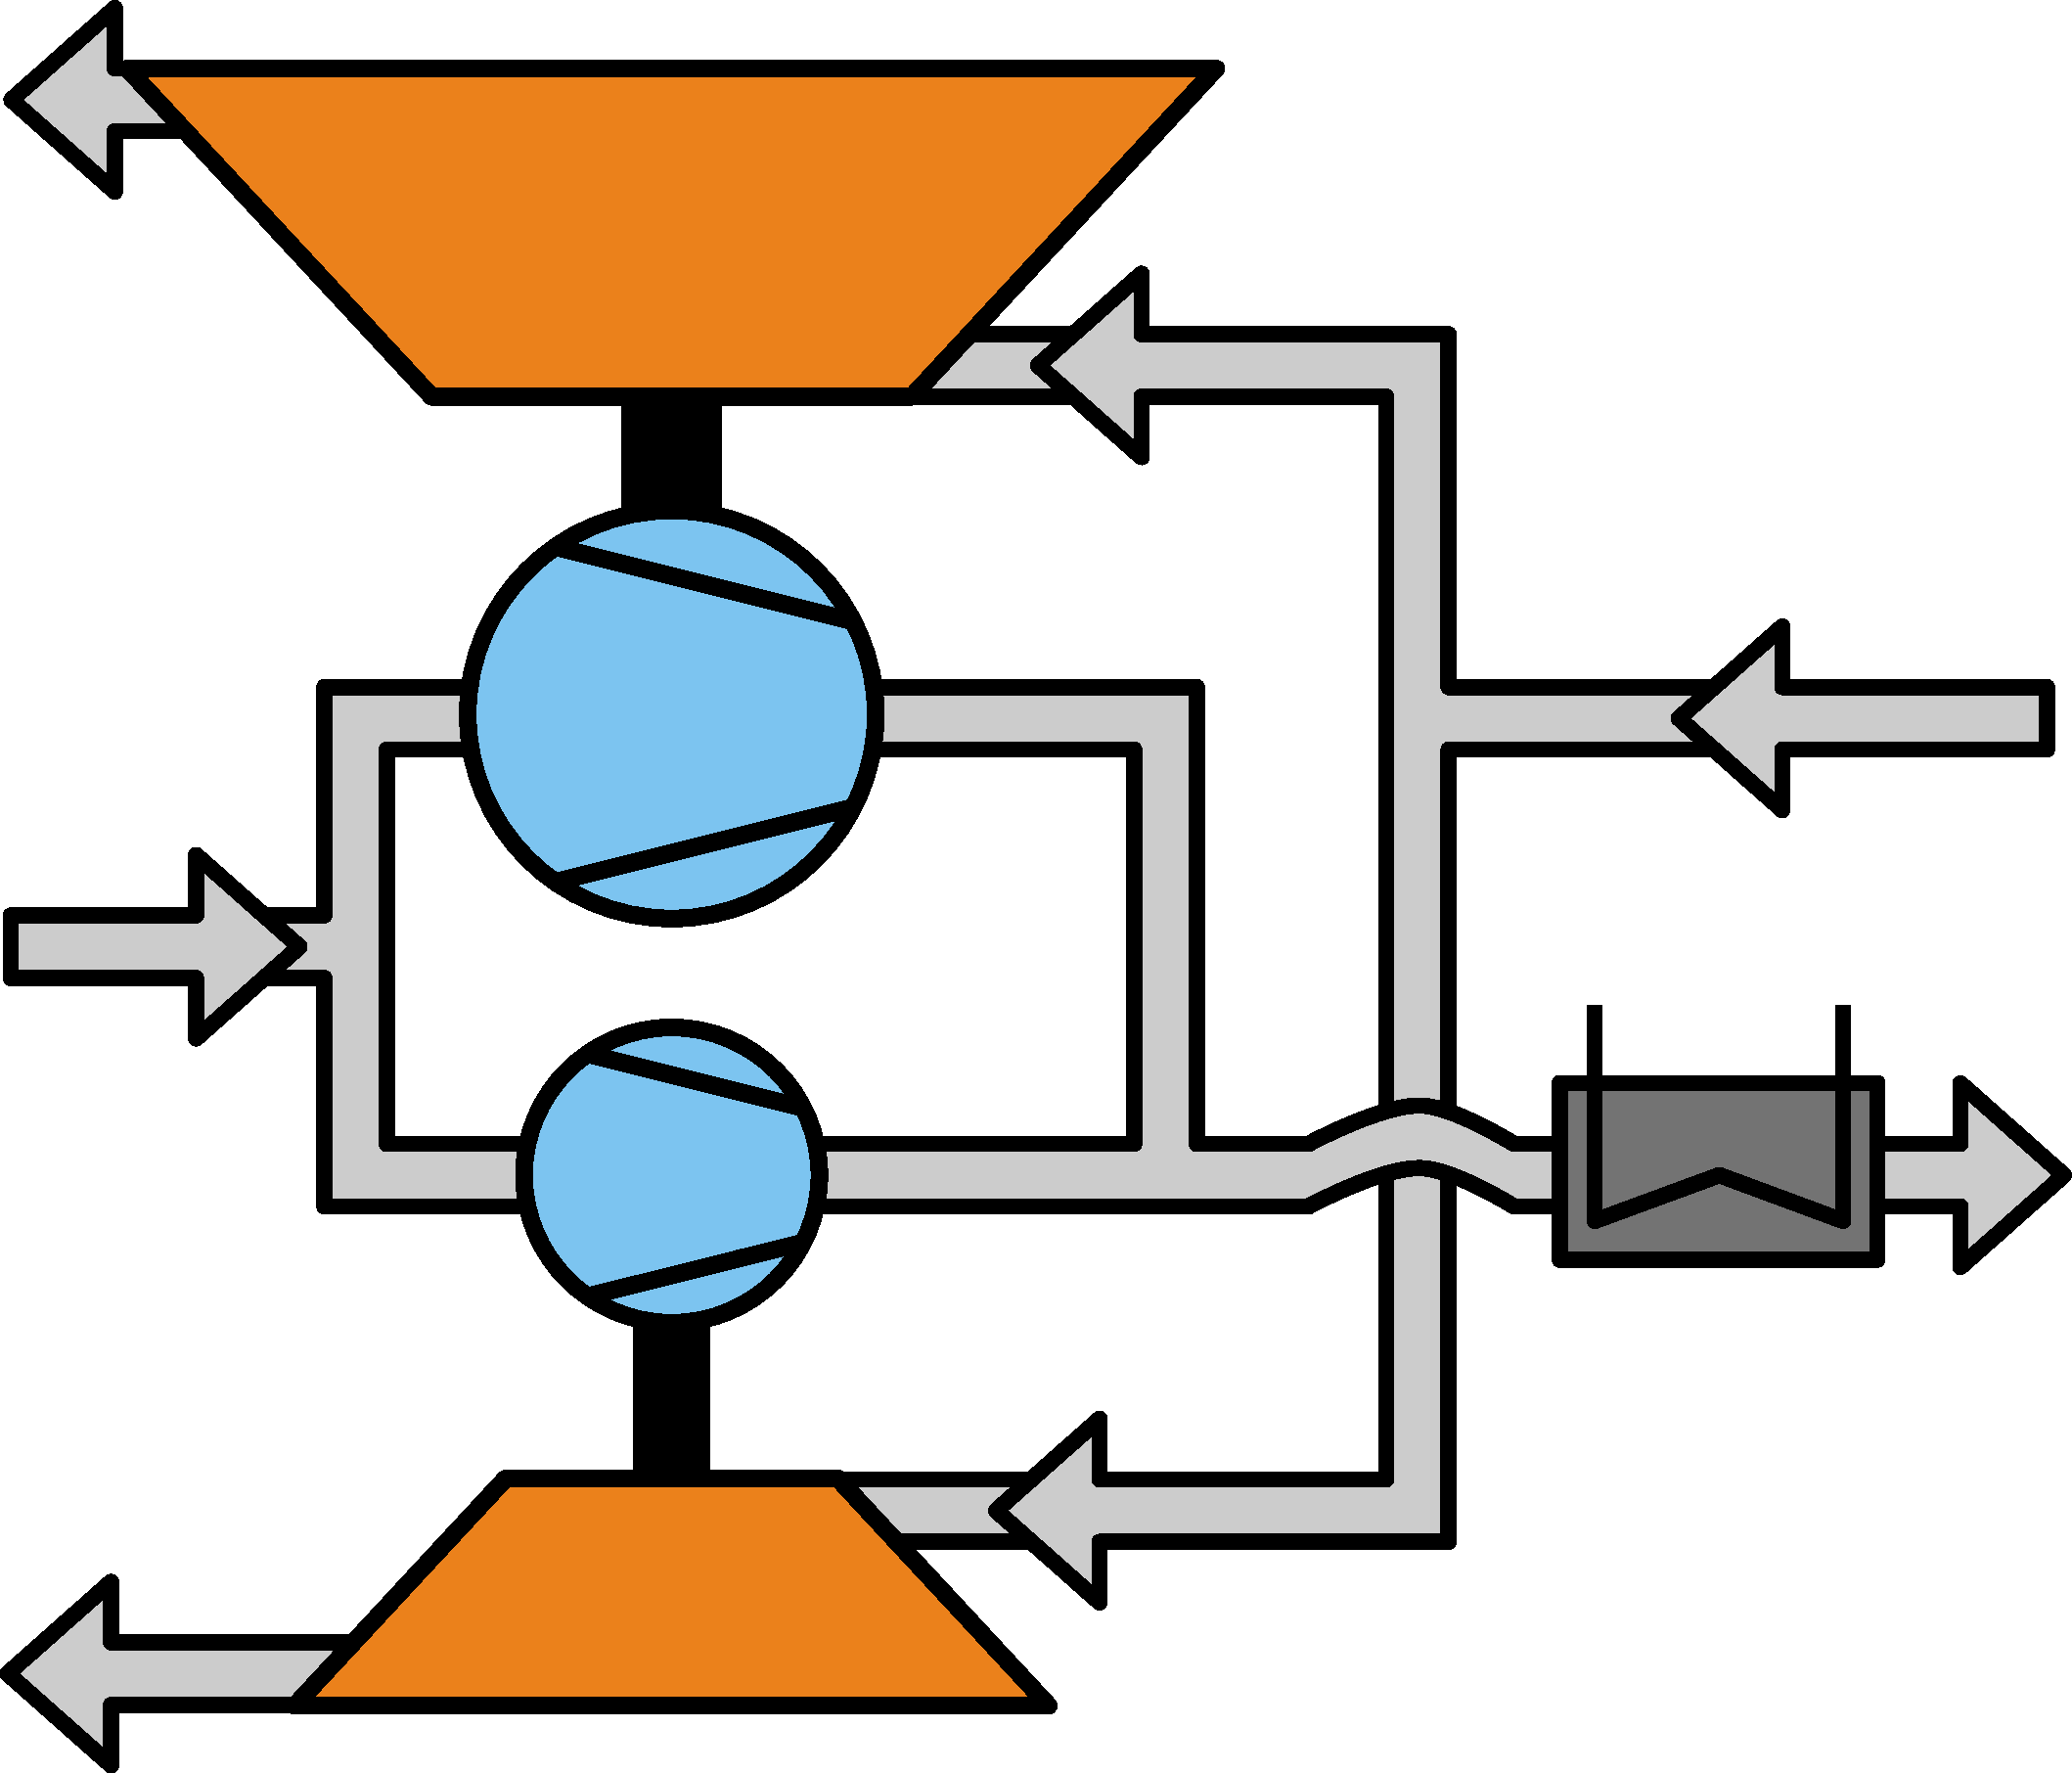
\includegraphics[width=0.3\textwidth]{turbo_parallel_pres}}%

\vspace*{\fill}

\visible<+->{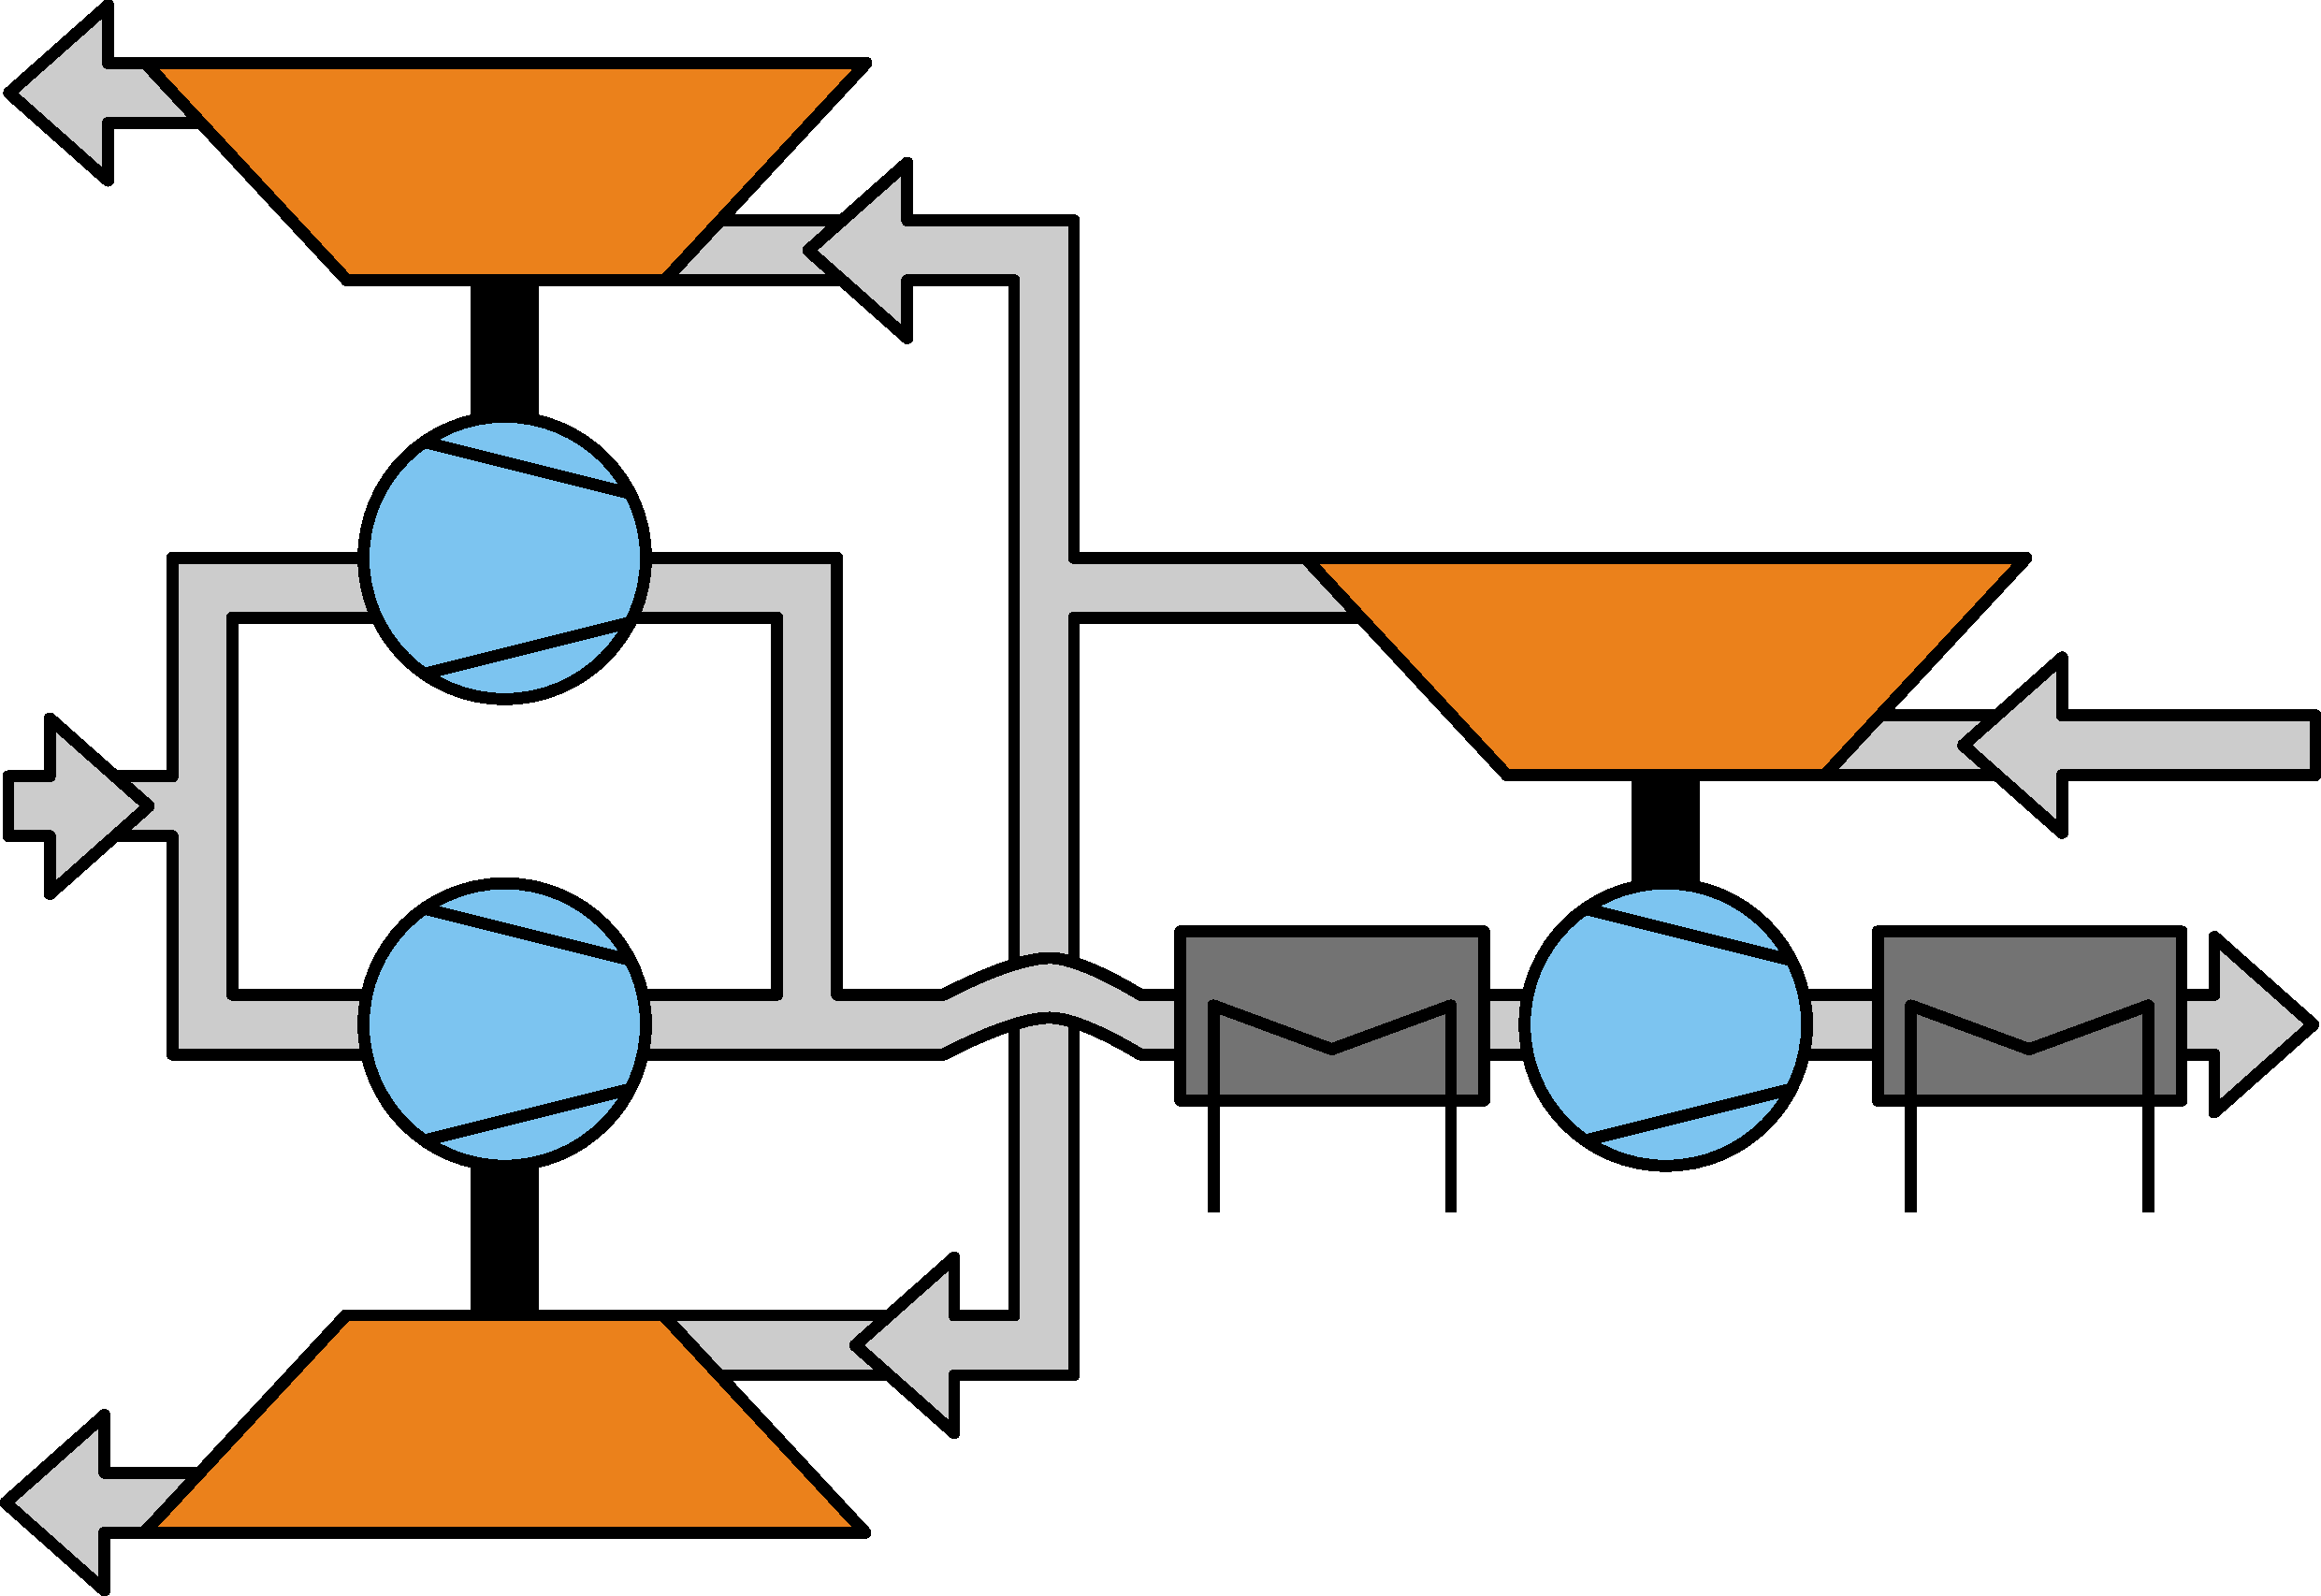
\includegraphics[width=0.4\textwidth]{turbo_triangle_pres}}%
\end{frame}
%%%%%%%%%%%%%%%%%%%%%%%%%%%%%%%%%%%%%%%%%%%%%%%%%%%%%%%%%%%%%%%%%%%%%%%%%%%%%%%%%%%%%%%%%%%
\begin{frame}<handout:0>[label=init-toc,plain, noframenumbering]%{Agenda}
% Now let them know the path to your end result so that they are prepared
\vspace*{\fill}

\tableofcontents[hideallsubsections]

\vspace*{\fill}
\end{frame}
%%%%%%%%%%%%%%%%%%%%%%%%%%%%%%%%%%%%%%%%%%%%%%%%%%%%%%%%%%%%%%%%%%%%%%%%%%%%%%%%%%%%%%%%%%%
\section{Core}
%%%%%%%%%%%%%%%%%%%%%%%%%%%%%%%%%%%%%%%%%%%%%%%%%%%%%%%%%%%%%%%%%%%%%%%%%%%%%%%%%%%%%%%%%%%
\begin{frame}<handout:1>[label=approach]{Reservoirs Approach}
 Using minipages; using 'columns' messed with overlay uncovering; using tabular messed with alignment
\begin{minipage}[c]{0.45\textwidth}
\begin{figure}
	\def\svgwidth{1\linewidth}
	\input{./images/reservoirs_model.pdf_tex}
\end{figure}
\end{minipage}
\pause
\hspace*{\fill}
\begin{minipage}[c]{0.45\textwidth}
\begin{enumerate}
\item \textbf{Isentropic conditions}
\begin{equation*}
\gls{pressure}\gls{specvolume}^{\gls{adexp}} = \text{\const{}}
\end{equation*}
\item \textbf{Mass conservation}
\begin{equation*}
\dot{\gls{mass}} = \gls{density} \vect{\gls{area}}{} \vect{\gls{velg}}{} = \text{\const{}}
\end{equation*}
\item \textbf{Energy conservation}
\begin{equation*}
0 = \dd{\gls{specenthalpy}} + \big(\vectcomp{\gls{velg}}{b}{}^2 - \vectcomp{\gls{velg}}{a}{}^2\big) / 2
\end{equation*}
\item \textbf{Ideal gas}
\begin{equation*}
\gls{pressure}\gls{specvolume} = \gls{specgascons}\gls{temperature}
\end{equation*}
\end{enumerate}
\end{minipage}
\end{frame}
%%%%%%%%%%%%%%%%%%%%%%%%%%%%%%%%%%%%%%%%%%%%%%%%%%%%%%%%%%%%%%%%%%%%%%%%%%%%%%%%%%%%%%%%%%%%
\subsection{Operating Conditions and Boundaries}
%%%%%%%%%%%%%%%%%%%%%%%%%%%%%%%%%%%%%%%%%%%%%%%%%%%%%%%%%%%%%%%%%%%%%%%%%%%%%%%%%%%%%%%%%%%%
\begin{frame}<handout:0>[label=operating-conditions]{Operating Conditions\autocites[43]{guzzella_introduction_2010}[72]{grieb_projektierung_2004}[32]{van_den_braembussche_design_2018}[1104\psq]{braunling_flugzeugtriebwerke:_2015}[25\psq]{grieb_verdichter_2009}[313]{bohl_technische_2014}[66]{herwig_stromungsmechanik:_2016}}
\centering
\begin{tikzpicture}[overlay, remember picture]%
\node at (0,1.8) (map) {%
\small
\def\svgwidth{0.45\textwidth}
\input{./images/boundary_map_pres.pdf_tex}
};
\pause
\node [below left = of map, text height=1.5ex] (similitude) {Similitude};
\node [right = 1em of similitude,text height=1.5ex] (mach) {\(\Mach \overset{!}{=} \text{\const}\)};
\draw[-stealth] (similitude) -- (mach);
\pause
\node [above right = 1ex and 1em of mach] (mach-mer) {meridional};
\node [below right = 1ex and 1em of mach] (mach-tan) {tangential};
\draw[-stealth] (mach) to[out=45,in=180] (mach-mer);
\draw[-stealth] (mach) to[out=315,in=180] (mach-tan);
\pause
\node [right = 1em of mach-mer] (mcor) {\(\dot{\gls{mass}}_{\gls{corrected}} \coloneqq \dot{\gls{mass}} \sqrt{\frac{\gls{temperature}_{\gls{total}}}{\gls{temperature}_{\gls{refstate}}}} \frac{\gls{pressure}_{\gls{refstate}}}{\gls{pressure}_{\gls{total}}}\)};
\node [right = 1em of mach-tan] (ncor) {\(\gls{rotspeed}_{\gls{corrected}} \coloneqq \gls{rotspeed}\sqrt{\frac{\gls{temperature}_{\gls{refstate}}}{\gls{temperature}_{\gls{total}}}}\)};
\draw[-stealth] (mach-mer) -- (mcor);
\draw[-stealth] (mach-tan) -- (ncor);
\end{tikzpicture}
\end{frame}
%%%%%%%%%%%%%%%%%%%%%%%%%%%%%%%%%%%%%%%%%%%%%%%%%%%%%%%%%%%%%%%%%%%%%%%%%%%%%%%%%%%%%%%%%%%%
\begin{frame}<handout:0>[label=instability-limit]{Instability Limit\autocites[41]{joos_stromungsmaschinen_2016}[1108]{braunling_flugzeugtriebwerke:_2015}[1]{dehner_simulation_2016}}
\centering
\begin{tikzpicture}[overlay,remember picture]
\node<+> at (0,1.8) (map) {%
\small
\def\svgwidth{0.45\textwidth}
\input{./images/boundary_map_pres.pdf_tex}%
};
\node<+-> at (0,1.8) (map) {%
\small
\def\svgwidth{0.45\textwidth}
\input{./images/boundary_map_pres_instabilities.pdf_tex}%
};
\node<+-> [below = of map] {\alert{Rotating stall} into \alert{surge} at \simplecross{}};
\end{tikzpicture}
\end{frame}
%%%%%%%%%%%%%%%%%%%%%%%%%%%%%%%%%%%%%%%%%%%%%%%%%%%%%%%%%%%%%%%%%%%%%%%%%%%%%%%%%%%%%%%%%%%%
\begin{frame}<handout:0>[label=diffusion-factor]{Diffusion Factor\autocites[41]{joos_stromungsmaschinen_2016}[1108]{braunling_flugzeugtriebwerke:_2015}}
\begin{overprint}
\begin{figure}
% When you're doing InkScape and not Tikz, you  might be forced to do uncovering of figures
% in ugly ways, as below.
% I don't know of a better approach!
\def\svgwidth{0.8\textwidth}%
\only<+>{\input{./images/stage_dimensions_compressor_pres.pdf_tex}}%
\only<+>{\input{./images/stage_dimensions_compressor_pres_smallsep.pdf_tex}}%
\only<+-6>{\input{./images/stage_dimensions_compressor_pres_largesep.pdf_tex}}%
\only<7->{\input{./images/stage_dimensions_compressor_pres_solidity.pdf_tex}}%
\end{figure}
\end{overprint}
\pause[\thebeamerpauses]%
\begin{equation*}
\gls{diffusionfactor} = 1 - \tikzmark{decel}\frac{ \vectcomp{\gls{velg}}{2}{} }{ \vectcomp{\gls{velg}}{1}{} } + \frac{\Delta\vectcomp{\gls{velg}}{}{\gls{tangential}}}{ \vectcomp{\gls{velg}}{1}{} }\tikzmark{redirection} \cdot \frac{1}{2\gls{solidity}}\tikzmark{solidity} > \num{0.6}
\end{equation*}
\pause
\begin{tikzpicture}[overlay, remember picture]% https://tex.stackexchange.com/a/254856/120853
\node [below left = of {pic cs:decel}] (decel-anno) {regular deceleration};
\draw[-stealth] (decel-anno) to [out=0,in=250] ([yshift=-2ex]{pic cs:decel});
\pause
\node [below right = of {pic cs:redirection}, align=center] (redirection-anno) {normalized\\redirection};
\draw[-stealth] (redirection-anno) to [out=180,in=290] ([yshift=-2ex]{pic cs:redirection});
\pause
\node [above right = 2.5ex and 2em of {pic cs:solidity}] (solidity-anno) {solidity \(\gls{solidity} = l/s\)};
\draw[-stealth] (solidity-anno) to [out=250,in=300] ([yshift=-1.5ex]{pic cs:solidity});
\end{tikzpicture}
\end{frame}
%%%%%%%%%%%%%%%%%%%%%%%%%%%%%%%%%%%%%%%%%%%%%%%%%%%%%%%%%%%%%%%%%%%%%%%%%%%%%%%%%%%%%%%%%%%%
\begin{frame}<handout:0>[label=choking]{Choking\autocites[43]{guzzella_introduction_2010}[310]{dixon_fluid_2014}}
\begin{minipage}{0.45\textwidth}
\small
\def\svgwidth{1\textwidth}
\only<+>{\input{./images/boundary_map_pres_choking.pdf_tex}}
\only<+->{\input{./images/boundary_map_pres.pdf_tex}}%
\end{minipage}%
\hspace{\fill}%
\begin{minipage}{0.4\textwidth}
\pause[\thebeamerpauses]
\raggedright
\(\dot{\gls{mass}}_{\gls{choke}} \overset{!}{=} \dot{\gls{mass}}_{\gls{choke}} (\gls{rotspeed})\), where \(\dd{\dot{\gls{mass}}_{\gls{choke}}}/\dd{\gls{rotspeed}} > 0\) and \(\gls{rotspeed} \propto \vectcomp{\gls{velc}}{}{}\)
\end{minipage}

\vspace*{\fill}

\pause
\begin{equation*}
\dot{\gls{mass}}_{\gls{choke}}(\vectcomp{\gls{velc}}{}{}) = \gls{area}\gls{density}\gls{sonic}_{0} \Bigg[\frac{2 + (\gls{adexp} - 1) (\vectcomp{\gls{velc}}{}{} / \gls{sonic}_{0})^2}{\gls{adexp} + 1}\Bigg]^{(\gls{adexp} + 1)/[2(\gls{adexp} - 1)]}
\end{equation*}
\end{frame}
%%%%%%%%%%%%%%%%%%%%%%%%%%%%%%%%%%%%%%%%%%%%%%%%%%%%%%%%%%%%%%%%%%%%%%%%%%%%%%%%%%%%%%%%%%%%
\subsection{Diffuser}
%%%%%%%%%%%%%%%%%%%%%%%%%%%%%%%%%%%%%%%%%%%%%%%%%%%%%%%%%%%%%%%%%%%%%%%%%%%%%%%%%%%%%%%%%%%%
\begin{frame}<handout:0>[label=diffuser]{Diffuser\autocites{stanitz_one-dimensional_1952}[7]{schneider_analytical_2015}[77\psqq]{schiff_preliminary_2013}[51\psq]{galvas_fortran_1973}{oh_optimum_1997}[441]{schiffmann_design_2010}[10]{japikse_assessment_1985}}
\begin{minipage}{0.5\textwidth}
\begin{figure}
\def\svgwidth{1\textwidth}
\input{./images/stanitz_force_balance.pdf_tex}
\end{figure}
\pause
\centering
\textrightarrow{} two coupled \glsxtrshortpl{ode}
\end{minipage}%
\hspace{\fill}%
\begin{minipage}{0.45\textwidth}
\pause
Key improvements:
\begin{itemize}
\item varying density
\item calibratable friction
\end{itemize}

\pause[\thebeamerpauses]
Assumptions:
\begin{itemize}
\item adiabatic
\item \(\gls{height} = \text{\const}\)
\item fully radial channel
\end{itemize}
\end{minipage}
\end{frame}
%%%%%%%%%%%%%%%%%%%%%%%%%%%%%%%%%%%%%%%%%%%%%%%%%%%%%%%%%%%%%%%%%%%%%%%%%%%%%%%%%%%%%%%%%%%%
\begin{frame}<handout:0>[label=diffuser-plot]{Diffuser Plot}
\begin{figure}
\pgfplotstableread{./data/stanitz_diffuser.csv}{\stanitzdiffusertable}%
\begin{tikzpicture}
\begin{axis}%
[%
minimalistic,%
width=0.8\textwidth,
height=0.8\textheight,
axis y line*=left,%
xlabel={\(\gls{radius}/\gls{radius}_{2}\)},%
x unit = {-},
ylabel={\(\Mach\), \(\gls{pressure}/\gls{pressure}_{2}\), \(\gls{temperature}/\gls{temperature}_{2}\), \(\gls{density}/\gls{density}_{2}\)},%
y unit = {-},
table/x={R_pres},%
ymin=0.4,
ymax=1.3,
ytick={0.4, 0.7, 1, 1.3},
xmin=1,
xmax=1.6,
title={Index \(2\): Diffuser Inlet},
]%
% Do this manually, node macro expansion in foreach/invokeforeach is weird
\addplot+ table [y=M] {\stanitzdiffusertable} node [pos = 0.2,fill=bg] {\(\Mach\)};
\addplot+ table [y=Pi] {\stanitzdiffusertable} node [pos = 0.9,fill=bg] {\(\gls{pressure}/\gls{pressure}_{2}\)};
\addplot+ table [y=Theta] {\stanitzdiffusertable} node [pos = 0.7,fill=bg] {\(\gls{temperature}/\gls{temperature}_{2}\)};
\addplot+ table [y=Rho] {\stanitzdiffusertable} node [pos = 0.8,fill=bg] {\(\gls{density}/\gls{density}_{2}\)};
\end{axis}%
\pause
\begin{axis}%
[%
minimalistic,%
width=0.8\textwidth,
height=0.8\textheight,
axis y line*=right,%
axis x line=none,%
ylabel = {abs.\ flow angle \gls{angabs}},%
y unit = {\degree},
cycle list shift=4,%
ymin=13,
ymax=15,
xmin=1,
xmax=1.6,
]%
\addplot+ table [x=R_pres, y=alpha] {\stanitzdiffusertable} node [pos = 0.6,fill=bg] {\gls{angabs}};%
\end{axis}%
\end{tikzpicture}
\end{figure}
\end{frame}
%%%%%%%%%%%%%%%%%%%%%%%%%%%%%%%%%%%%%%%%%%%%%%%%%%%%%%%%%%%%%%%%%%%%%%%%%%%%%%%%%%%%%%%%%%%
\section{Supplementary}
%%%%%%%%%%%%%%%%%%%%%%%%%%%%%%%%%%%%%%%%%%%%%%%%%%%%%%%%%%%%%%%%%%%%%%%%%%%%%%%%%%%%%%%%%%%
\begin{frame}<handout:0>[label=gas-properties]{Gas Properties\autocites[15]{dixon_fluid_2014}{shomate_method_1954}{buck_new_1981}{sutherland_viscosity_1893}{vogel_uber_1914}[2]{davidson_simple_1993}{graham_motion_1846}}
\begin{center}
\begin{tabular}{c@{\hspace{2em}}c}
\begin{tikzpicture}
\begin{axis}[%
minimalistic,%
ylabel={\(c_{p,\text{air}}\)},
y unit = {\joule\per\kilogram\per\kelvin},
xlabel={\gls{temperature}},%
x unit = {\kelvin},
domain=300:700,
ymin = 1000,
ymax = 1100,
ytick = {1000, 1050, 1100},% Specify manually due to weird rounding
title={Caloric properties},
]
	\addplot+{cpm(x-273.15)/0.0289524} node [pos = 0.3,fill=bg,inner sep=0.5pt,sloped] {\tiny \(c_{p,\text{air}}\)};%
\end{axis}
%\pause
\begin{axis}[%https://tex.stackexchange.com/a/31504/120853
minimalistic,%
axis y line*=right,%
axis x line=none,%
ylabel={\gls{adexp}},%
y unit = {-},
cycle list shift=1,
domain = 300:700,
ymin = 1.35,
ymax = 1.4,
]
	\addplot+{cpm(x-273.15)/(cpm(x-273.15)-8.3145)} node [pos = 0.3,fill=bg,inner sep=0.5pt,sloped] {\tiny \gls{adexp}};
\end{axis}
\end{tikzpicture}
\pause
&
\begin{tikzpicture}
\begin{axis}[%
minimalistic,
ylabel={\(\gls{dynvisc}_{\text{air}}\)},
y unit = {\pascal\second},
y SI prefix = {micro},
xlabel={\gls{temperature}},
x unit = {\kelvin},
ymin = 10,
ymax = 50,
domain=200:1000,
xtick={200,600,1000},
title={Viscosity},
]%
\addplot+ {10^6 * (0.2093*muoxy(x) + 0.7810*munit(x) + 0.0093*muar(x) + 0.0004*mucoo(x))};% Mixing using Graham approach, from Sutherland equations
\end{axis}
\end{tikzpicture}\pause\\
\multicolumn{2}{c}{%
\begin{tikzpicture}
\begin{axis}[%
minimalistic,%
ylabel={\(\gls{pressure}^{\ast}_{\chcpd{H2O}}\)},%
y unit = {\bar},
xlabel={\gls{temperature}},%
x unit = {\kelvin},
domain=273:373,
ymin = 0,
ymax = 1.1,
title={Phase change},
]
\addplot+ {611.21*exp((18.678-((x-273.15)/234.5))*((x-273.15)/(257.14+x-273.15)))/1e5};
\end{axis}
\end{tikzpicture}
}%
\end{tabular}
\end{center}
\end{frame}
%%%%%%%%%%%%%%%%%%%%%%%%%%%%%%%%%%%%%%%%%%%%%%%%%%%%%%%%%%%%%%%%%%%%%%%%%%%%%%%%%%%%%%%%%%%%
\begin{frame}<handout:0>[label=gas-volumes]{Gas Volumes\autocites{eriksson_modeling_2007}[30]{guzzella_introduction_2010}{hendricks_isothermal_2001}{mathworks_constant_2018}}
\centering
\begin{figure}
	\def\svgwidth{0.8\textwidth}
	\input{./images/gas_volume.pdf_tex}
\end{figure}
\pause
\textrightarrow{} two coupled \glsxtrshortpl{ode} for \(\gls{pressure}(\gls{time})\) and \(\gls{temperature}(\gls{time})\)
\end{frame}
%%%%%%%%%%%%%%%%%%%%%%%%%%%%%%%%%%%%%%%%%%%%%%%%%%%%%%%%%%%%%%%%%%%%%%%%%%%%%%%%%%%%%%%%%%%%
\section{Third Section}
%%%%%%%%%%%%%%%%%%%%%%%%%%%%%%%%%%%%%%%%%%%%%%%%%%%%%%%%%%%%%%%%%%%%%%%%%%%%%%%%%%%%%%%%%%%%
%%%%%%%%%%%%%%%%%%%%%%%%%%%%%%%%%%%%%%%%%%%%%%%%%%%%%%%%%%%%%%%%%%%%%%%%%%%%%%%%%%%%%%%%%%%%
\begin{frame}{More content needed!}
	More content...
\end{frame}
%%%%%%%%%%%%%%%%%%%%%%%%%%%%%%%%%%%%%%%%%%%%%%%%%%%%%%%%%%%%%%%%%%%%%%%%%%%%%%%%%%%%%%%%%%%%
%\miniframesoff
%%%%%%%%%%%%%%%%%%%%%%%%%%%%%%%%%%%%%%%%%%%%%%%%%%%%%%%%%%%%%%%%%%%%%%%%%%%%%%%%%%%%%%%%%%%%
%% New empty section; neither in ToC nor navigation.
%% Anything after is not highlighted in the navigation
%% https://tex.stackexchange.com/a/66633/120853
\section*{}
%%%%%%%%%%%%%%%%%%%%%%%%%%%%%%%%%%%%%%%%%%%%%%%%%%%%%%%%%%%%%%%%%%%%%%%%%%%%%%%%%%%%%%%%%%%%
\begin{frame}<handout:0>[label=outro]{Outro}
\begin{itemize}
\item we learned this
\item and that
\end{itemize}
\end{frame}
\begin{frame}<handout:0>[standout,plain]{}
Thank you.
\end{frame}
%%%%%%%%%%%%%%%%%%%%%%%%%%%%%%%%%%%%%%%%%%%%%%%%%%%%%%%%%%%%%%%%%%%%%%%%%%%%%%%%%%%%%%%%%%%%
%%%%%%%%%%%%%%% Repeat slides for easy access without scrolling through animations
%%%%%%%%%%%%%%% No idea how to access \againframe<last frame>, therefore manual adjusting
%%%%%%%%%%%%%%%%%%%%%%%%%%%%%%%%%%%%%%%%%%%%%%%%%%%%%%%%%%%%%%%%%%%%%%%%%%%%%%%%%%%%%%%%%%%%
\setcounter{framenumber}{0}% Reset to zero, so it starts from 1
%\againframe[standout,plain,noframenumbering]{attention-getter}%
\againframe<3|handout:0>{upshot}%
%%%%%%%%%%%%%%%%%%%%%%%%%%%%%%%%%%%%%%%%%%%%%%%%%%%%%%%%%%%%%%%%%%%%%%%%%%%%%%%%%%%%%%%%%%%%
%%%%%%%%%%%%%%% Appendix with plain style etc.
%%%%%%%%%%%%%%%%%%%%%%%%%%%%%%%%%%%%%%%%%%%%%%%%%%%%%%%%%%%%%%%%%%%%%%%%%%%%%%%%%%%%%%%%%%%%
\appendix
\beamerdefaultoverlayspecification{}% Reset to default of <*> (no piecewise uncovering)
\addtobeamertemplate{frametitle}{\vspace*{-\headheight}}{}% Shift title upwards by height of navigation; https://tex.stackexchange.com/a/321889/120853
\begin{frame}<handout:0>[standout,plain]
Appendix
\end{frame}
%%%%%%%%%%%%%%%%%%%%%%%%%%%%%%%%%%%%%%%%%%%%%%%%%%%%%%%%%%%%%%%%%%%%%%%%%%%%%%%%%%%%%%%%%%%%
%%%%%%%%%%%%%%% Back-Up Slides
%%%%%%%%%%%%%%%%%%%%%%%%%%%%%%%%%%%%%%%%%%%%%%%%%%%%%%%%%%%%%%%%%%%%%%%%%%%%%%%%%%%%%%%%%%%%
\begin{frame}<handout:0>[label=pressure-magnitude-development]{Pressure Magnitude Development}
\begin{figure}
\begin{tikzpicture}
[%
every path/.style={%https://tex.stackexchange.com/a/302931/120853
	thick,%
	>=stealth',%
	shorten <=2pt,%
	shorten >=2pt,%
},%
outflow/.style = {->, bend right, dashdotted, line width = 2pt},%
conversion/.style = {->, dashed, line width = 2pt},%
physflow/.style = {->, bend right},%
every node/.style = {draw, circle},%
]%
\node (p2) {\(\gls{pressure}_2\)};
\node [above left = of p2, fill = mLightBrown] (prot) {\(\gls{pressure}_{\gls{rotating}}\)} edge[outflow] (p2);
\node [below = 17ex of prot, fill = mLightBrown] (p1) {\(\gls{pressure}_1\)} edge[conversion] (prot);
\node [above left = of p1] (p0) {\(\gls{pressure}_0\)} edge[outflow] (p1);
\draw [physflow] (p0) edge (p2);
\end{tikzpicture}
\end{figure}
\end{frame}
%%%%%%%%%%%%%%%%%%%%%%%%%%%%%%%%%%%%%%%%%%%%%%%%%%%%%%%%%%%%%%%%%%%%%%%%%%%%%%%%%%%%%%%%%%%%
\begin{frame}<handout:0>[label=molar-masses]{Molar Masses}
\begin{table}
\begin{tabular}{@{}lcS[table-format=1.6]@{}}
\toprule
	Element & Symbol & {\(\gls{molarmass}\,/\,\si{\kilogram\per\mole}\)}\\
\midrule
	Carbon & \chcpd{C}   & 0.012011\\
	Hydrogen & \chcpd{H}  & 0.001008\\
	Sulphur & \chcpd{S}   & 0.032065\\
	Oxygen & \chcpd{O}  & 0.015999\\
	Nitrogen & \chcpd{N}  & 0.014007\\
	Argon & \chcpd{Ar} & 0.039948 \\
\bottomrule
\end{tabular}
\end{table}%
\end{frame}
%%%%%%%%%%%%%%%%%%%%%%%%%%%%%%%%%%%%%%%%%%%%%%%%%%%%%%%%%%%%%%%%%%%%%%%%%%%%%%%%%%%%%%%%%%%%
\begin{frame}<handout:0>[label=gas-properties-der]{Gas Properties Derivation}
\begin{center}
\begin{tikzpicture}
% Top row of gases:
\node (O2) {\chcpd{O2}};
\node [right = of O2] (N2) {\chcpd{N2}};
\node [right = of N2] (Ar) {\chcpd{Ar}};
\node [right = of Ar] (CO2) {\chcpd{CO2}};
\node [right = of CO2] (H2O) {\chcpd{H2O}};
\node [right = of H2O] (SO2) {\chcpd{SO2}};
% Composition:
\node [below = of $(Ar)!0.5!(CO2)$] (composition) {\alert<6->{\textbf{gas composition}}};
% Connect parts to composition:
\draw[-stealth] [out=270] (O2) to [in=180] (composition);
\draw[-stealth] [out=270] (N2) to [in=135] (composition);
\draw[-stealth] [out=270] (Ar) to [in=90] (composition);
\draw[-stealth] [out=270] (CO2) to [in=90] (composition);
\draw[-stealth] [out=270] (H2O) to [in=45] (composition);
\draw[-stealth] [out=270] (SO2) to [in=0] (composition);
\pause
% Bottom part:
\node [below = of composition] (molmass) {\alert<6->{\gls{molarmass}}};
\node [below left = of molmass, align = center] (cpm) {\alert<6->{\(c_{p,\text{m}}(\gls{temperature})\)}};
\draw[-stealth] (composition) to (molmass);
\draw[-stealth] [out=270] (composition) to [in=90] node [midway,sloped,fill=bg] {\color{gray}\scriptsize\name{Shomate}\autocite{shomate_method_1954}} (cpm);
\pause
% Bottom right part:
\node [right = of molmass] (gascons) {\gls{specgascons}};
\draw[-stealth] (molmass) -- (gascons) node [pos = 0.5, above] {\(R_{\text{m}}\)};
\pause
\node [below = of gascons] (cp) {\(\gls{specheatcappres}(\gls{temperature})\)};
\draw[-stealth] (cpm) -- (cp);
\draw[-stealth] [out=270] (molmass) to [in=180] (cp);
\pause
\node [right = 5em of $(gascons)!0.5!(cp)$] (result) {\(\gls{specheatcapvol}(\gls{temperature})\) and \(\gls{adexp}(\gls{temperature})\)};
\draw[-stealth] [out=0] (gascons) to [in=180] (result);
\draw[-stealth] [out=0] (cp) to [in=180] (result);
\end{tikzpicture}
\end{center}
\end{frame}
%%%%%%%%%%%%%%%%%%%%%%%%%%%%%%%%%%%%%%%%%%%%%%%%%%%%%%%%%%%%%%%%%%%%%%%%%%%%%%%%%%%%%%%%%%%%
\begin{frame}<handout:0>[label=fuel-and-combustion]{Fuel and Combustion}
\begin{tikzpicture}
% Top row of fuel components:
\node (ash) {Ash};
\node [right = of ash] (C) {\chcpd{C}};
\node [right = of C] (H) {\chcpd{H}};
\node [right = of H] (S) {\chcpd{S}};
\node [right = of S] (O) {\chcpd{O}};
\node [right = of O] (N) {\chcpd{N}};
\node [right = of N] (H2O) {\chcpd{H2O}};
% Composition:
\node [below = of S] (composition) {\textbf{fuel composition}};
% Connect parts to composition:
\foreach[count=\i from 0, evaluate=\i as \x using int(\i*30)] \y in {H2O, N, O, S, H, C, ash}{%
	\draw[-stealth] [out=270] (\y) to [in=\x] (composition);
}%
\pause
% Inferior Heating Value:
\node [below = of composition] (hi) {\(\gls{heatingvalue}_{\gls{component}}\)};
\draw[-stealth] (composition) -- (hi) node [pos=0.5,fill=bg] {\color{gray}\scriptsize\name{Boie}\autocite{dubbel_taschenbuch_2007}};
\pause
% Left flank:
\node [below left = of composition] (mu0O2) {\(\gls{massperfuel}_{\gls{stoichiometric},\chcpd{O2}}\)};
\draw[-stealth] [out=225] (composition) to [in=90] (mu0O2);
\node [below = of mu0O2] (mu0air) {\(\gls{massperfuel}_{\gls{stoichiometric},\text{air}}\)};
\draw[-stealth] (mu0O2) -- (mu0air) node [pos=0.5,fill=bg] {\color{gray}\scriptsize\(\gls{massfrair}_{\chcpd{O2}}\)};
\pause
% Helper coordinate:
\coordinate (help1) at (ash|-mu0air);
% Bottom left corner:
\node [below = of help1] (mu0exh) {\(\gls{massperfuel}_{\gls{stoichiometric},\text{exh}}\)};
%\begin{scope}[on background layer]% Buggy with beamer overlays
	\draw[-stealth] (ash) -- (mu0exh);
%\end{scope}
\draw[-stealth] [out=180] (mu0air) to [in=90] (mu0exh);
\pause
% With Lambda:
\node at (mu0exh-|composition) (muexh) {\(\gls{massperfuel}_{\text{exh}}\)};
\draw[-stealth] (mu0exh) -- (muexh) node [pos=0.5,fill=bg] {\color{gray}\scriptsize\(\gls{fuelairratio}\)};
\pause
% Resulting mass composition:
\node[right = of muexh] (gamma) {\(\gls{massfr}_{\gls{component},\text{exh}}\)};
\draw[-stealth] (muexh) -- (gamma);
\draw[-stealth] [out=315] (composition) to [in=180] (gamma);
% Volumetric composition:
\node[right = of gamma] (phi) {\(\gls{volfr}_{\gls{component},\text{exh}}\)};
\draw[-stealth] (gamma) -- (phi) node [pos=0.5,fill=bg] {\color{gray}\scriptsize\(\gls{molarmass}\)};
\end{tikzpicture}
\end{frame}
%%%%%%%%%%%%%%%%%%%%%%%%%%%%%%%%%%%%%%%%%%%%%%%%%%%%%%%%%%%%%%%%%%%%%%%%%%%%%%%%%%%%%%%%%%%%
%%%%%%%%%%%%%%% References
%%%%%%%%%%%%%%%%%%%%%%%%%%%%%%%%%%%%%%%%%%%%%%%%%%%%%%%%%%%%%%%%%%%%%%%%%%%%%%%%%%%%%%%%%%%%
\begin{frame}<handout:0>[standout,plain]
References
\end{frame}
\begin{frame}<handout:0>[allowframebreaks]{References}% Note that allowframebreaks won't work with label
\setbeamertemplate{bibliography item}{\insertbiblabel}% Print label/number instead of icon
\renewcommand*{\bibfont}{\tiny}% https://tex.stackexchange.com/a/343/120853
\printbibliography
\end{frame}
\begin{frame}<handout:0>[standout,plain]
End of slides.
\end{frame}
%%%%%%%%%%%%%%%%%%%%%%%%%%%%%%%%%%%%%%%%%%%%%%%%%%%%%%%%%%%%%%%%%%%%%%%%%%%%%%%%%%%%%%%%%%%%
%%%%%%%%%%%%%%% Abstract
%%%%%%%%%%%%%%%%%%%%%%%%%%%%%%%%%%%%%%%%%%%%%%%%%%%%%%%%%%%%%%%%%%%%%%%%%%%%%%%%%%%%%%%%%%%%
\begin{frame}<handout:0>[allowframebreaks,squeeze]{Abstract}% Squeeze: reduce vert. space
\tiny
\justifying
% https://tex.stackexchange.com/a/40887/120853
% Starred variant: reset existing font
\setbeamerfont*{itemize/enumerate body}{size=\tiny}
\setbeamerfont*{itemize/enumerate subbody}{parent=itemize/enumerate body}
\setbeamerfont*{itemize/enumerate subsubbody}{parent=itemize/enumerate body}
\Blindtext

\begin{itemize}
	\item we found out this
	\item and also that!
\end{itemize}
\end{frame}
%%%%%%%%%%%%%%%%%%%%%%%%%%%%%%%%%%%%%%%%%%%%%%%%%%%%%%%%%%%%%%%%%%%%%%%%%%%%%%%%%%%%%%%%%%%%
%%%%%%%%%%%%%%% Other
%%%%%%%%%%%%%%%%%%%%%%%%%%%%%%%%%%%%%%%%%%%%%%%%%%%%%%%%%%%%%%%%%%%%%%%%%%%%%%%%%%%%%%%%%%%%
\begin{frame}<handout:0>[label=gitmeta]{Document Information}
\DeclareUrlCommand\EscWrapper{\urlstyle{tt}}%https://tex.stackexchange.com/a/20891/120853
{%
\color{gray}
\tiny
\textcolor{gray!80}{Compiled on \DTMnow{}.}

\scriptsize
{\ttfamily\bfseries\jobname{}
% Expand Argument first, then wrap into special command to escape chars
\expandafter\EscWrapper\expandafter{\GitVersion}
(\expandafter\EscWrapper\expandafter{\GitShorthash})}\\[\baselineskip]

\prettybanner{}.
\hologo{\fmtname} (\fmtversion) with \texttt{glossaries-extra} (\texttt{bib2gls}) and \hologo{biber}.

Theme adapted from \url{https://github.com/matze/mtheme}.
}%
\end{frame}
\begin{frame}<handout:0>[standout,plain]
End of document.
\end{frame}
\end{document}